% \documentclass{beamer}
% % početak: može, ali ne mora
% \usetheme{metropolis} % {default} {Goettingen} {Copenhagen}
% \setbeamercovered{transparent} % ovo je važno za dinamiku
% \usecolortheme{default} % {seahorse}{rose}{wolverine}{infolines}
% % kraj: može, ali ne mora
% \usepackage[utf8]{inputenc}
% \usepackage[T1, T2A]{fontenc}
% \usepackage[serbianc]{babel}
% \usepackage{datetime}
% \title[prezentacija]{\huge prezentacija}
% \date{\today}
% \begin{document}
% \begin{frame}
% \titlepage
% \end{frame}
% \end{document}

\documentclass{beamer}
\usetheme{metropolis}           % Use metropolis theme {metropolis}

\setbeamercovered{transparent}

\usepackage[utf8]{inputenc}
\usepackage[T1, T2A]{fontenc}
\usepackage[serbianc]{babel}
\usepackage{datetime}

\usepackage[labelformat=empty]{caption}
%%%%%%%%%%%%%%%%%%%%%%%%%%%
\usepackage{amsmath}
\usepackage{mathtools}
\DeclarePairedDelimiter\ceil{\lceil}{\rceil}
\DeclarePairedDelimiter\floor{\lfloor}{\rfloor}
%%%%%%%%%%%%%%%%%%%%%%%%%%%
\usepackage{float}
\usepackage{minted}
\usepackage{verbatim}
\usepackage{cite}

\bibliographystyle{ieeetr}
%\setlength{\bibsep}{0.0pt}

\hypersetup{
    colorlinks=true,
    linkcolor=black,
    citecolor=black,
    filecolor=magenta,      
    urlcolor=cyan,
}
\makeatletter
\g@addto@macro\UrlBreaks{\do\-}
%\g@addto@macro{\UrlBreaks}{\UrlOrds}
\makeatother


\AtBeginSection[]
{
  \begin{frame}
    \frametitle{Садржај}
    \tableofcontents[currentsection]
  \end{frame}
}

\title{\alert{Дипломски рад}\\
Детекција карата за игру коришћењем
YOLO алгоритма за детекцију објеката}
%\date{\today}
\date{18. септембар 2020.}
\author{\alert{Студент: Алекса Величковић 576/2015} \\
Професор: др Владимир Миловановић}
\institute{Универзитет у Крагујевцу \\
Факултет инжењерских наука}

% logo of my university
\titlegraphic{%
  \begin{picture}(0,0)
    \put(305,-165){\makebox(0,0)[rt]{
\includegraphics[scale=0.22]{slike/grb.jpg}}}
  \end{picture}}


\begin{document}
\maketitle

\section{Увод}

\begin{frame}
\frametitle{YOLO алгоритам и програмски оквир Darknet}

\begin{itemize}
 \item YOLO (You Only Look Once) - алгоритам за детекцију објеката у реалном времену
 \item Darknet је програмски оквир и представља имплементацију YOLO алгоритма
\end{itemize}

\begin{figure}[H]
  \centering
      
\includegraphics[scale=0.2]{slike/yologo.png} \\
      
\includegraphics[scale=0.15]{slike/darknet.png}
\end{figure}

\end{frame}

%%%%%%%%%%%%%%%%%%%%%%%%%%%%%%%%%%%%%%%%%%%%%%%%%%%%%%
\section{Припрема тренинг скупа}
%%%%%%%%%%%%%%%%%%%%
\subsection{Добијање слика из видеа}
\begin{frame}
\frametitle{Добијање слика из видеа}

\begin{itemize}
 \item Шаблон за издвајање карте са снимка
 \item Функција \alert{extract\_card()} издваја карту са прослеђене слике 
 \begin{itemize}
  \item Провера замућења слике; смањење шума; издвајање ивица (прелаза)
  са слике и налажење контура (спаја све тачке дуж границе,
  исте боје и интензитета)
  \item Требало би да је највећа контура карта;
  проверава се да ли је приближно правоугаоног облика
  \item Простор унутар контуре се претвара у правоугаоник
  димензија карте (шаблона)
 \end{itemize}

\end{itemize}
\begin{figure}[H]
  \centering
      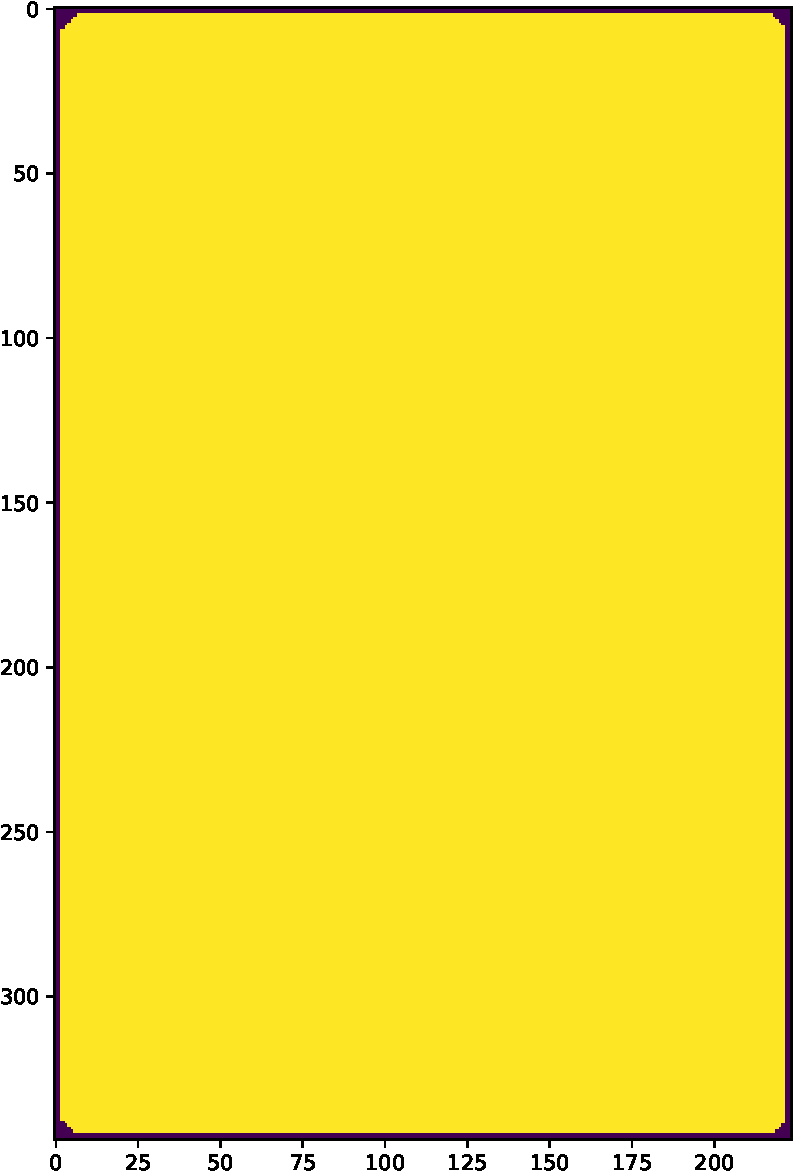
\includegraphics[scale=0.15]{slike/alphamask.pdf} \hspace{1.2cm}
      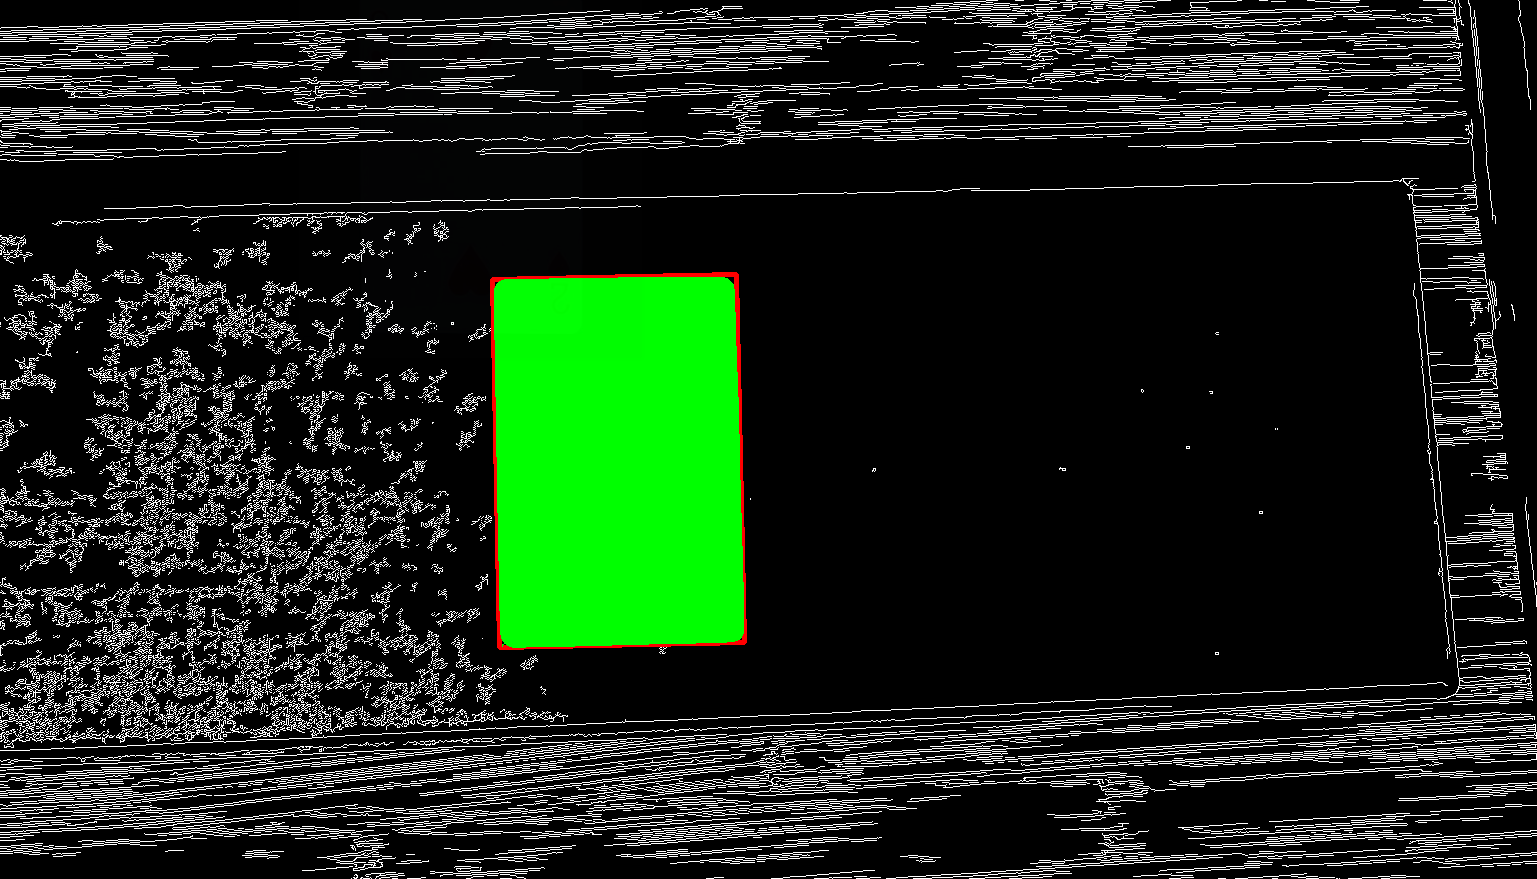
\includegraphics[scale=0.12]{slike/extract_2hCrop.png}
 \end{figure}
\end{frame}
%%%%%%%%%%%%%%%%%%%%
\subsection{Означавање знака и броја карте на слици}
\begin{frame}
\frametitle{Означавање знака и броја карте на слици}
\begin{itemize}
 \item Дефинисане су позиције ћошкова
 правоугаоника који окружује знак и број карте
\end{itemize}
\begin{figure}[H]
  \centering
      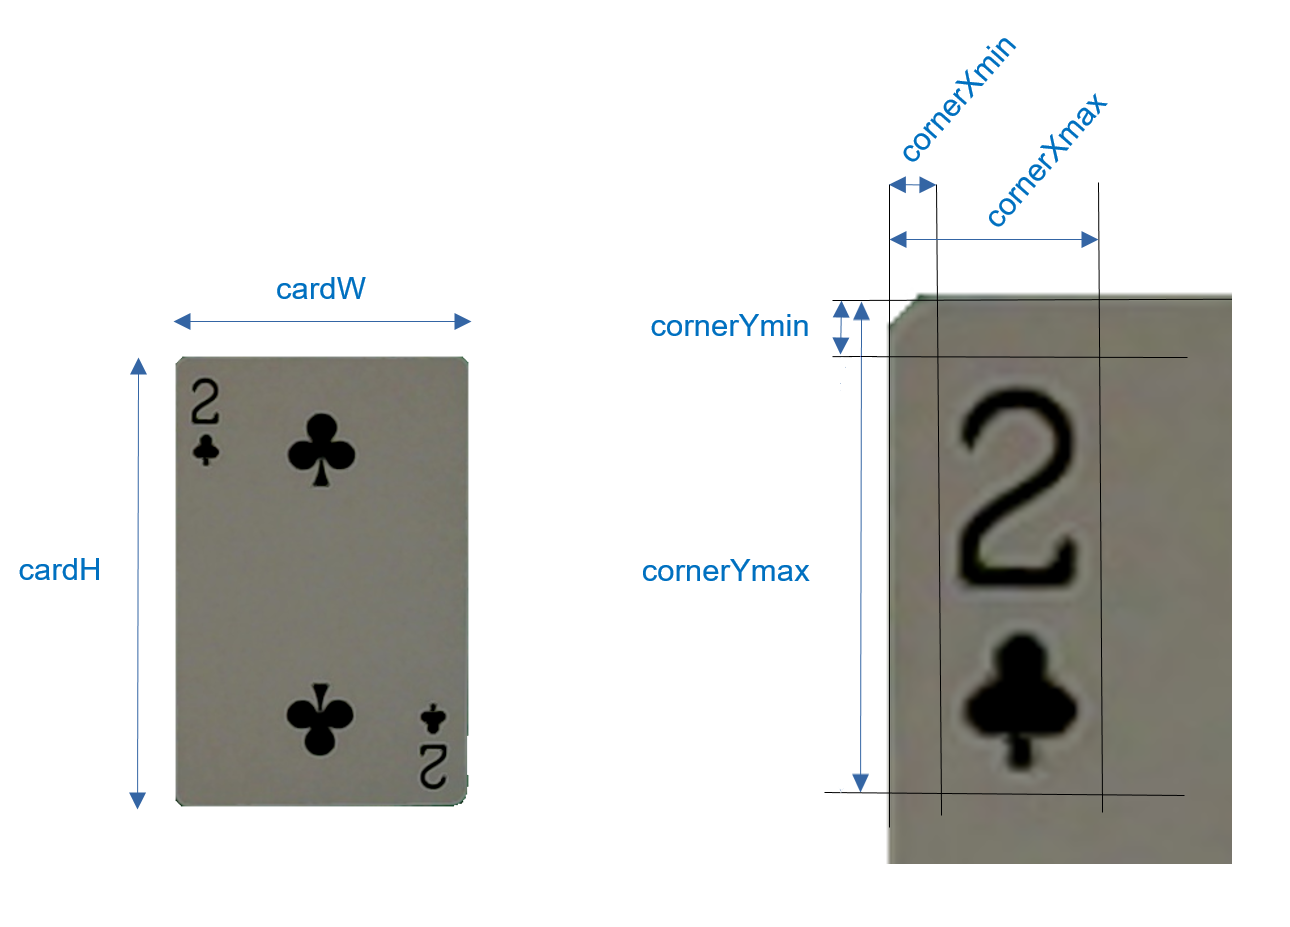
\includegraphics[scale=0.27]{slike/measures.png}
 \end{figure}
\end{frame}

\begin{frame}
\frametitle{Означавање знака и броја карте на слици}
\begin{itemize}
 \item Функција \alert{find\_hull()} унутар правоугаоника
 налази полигон (контуру), унутар кога се налазе знак и број
 \begin{itemize}
  \item Издваја се део слике карте означен позицијама правоугаоника;
  ивице (прелази) се „појачавају”; налазе се контуре и конвексни
  полигони око њих
  \item Врше се провере да ли је: контура већа од минимално дефинисане
  (\alert{min\_area});
  однос површина контуре и конвексног полигона
  већи од минималног (\alert{min\_solidity}) и
  да ли је тежиште контуре близу центра правоугаоника
 \end{itemize}

\end{itemize}
\begin{figure}[H]
  \centering
      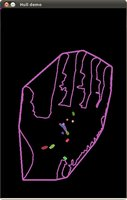
\includegraphics[scale=0.4]{slike/Hull_Result.jpg}
 \end{figure}
\end{frame}

\begin{frame}
\frametitle{Означавање знака и броја карте на слици}
\begin{itemize}
 \item Све контуре су спојене у једну и одеђен је полигон око ње
 \item Уколико је површина полигона у границама минималне и
 максималне дефинисане вредности, позцију полигона треба дефинисати
 у односу ивицу карте
\end{itemize}
\begin{figure}[H]
  \centering
      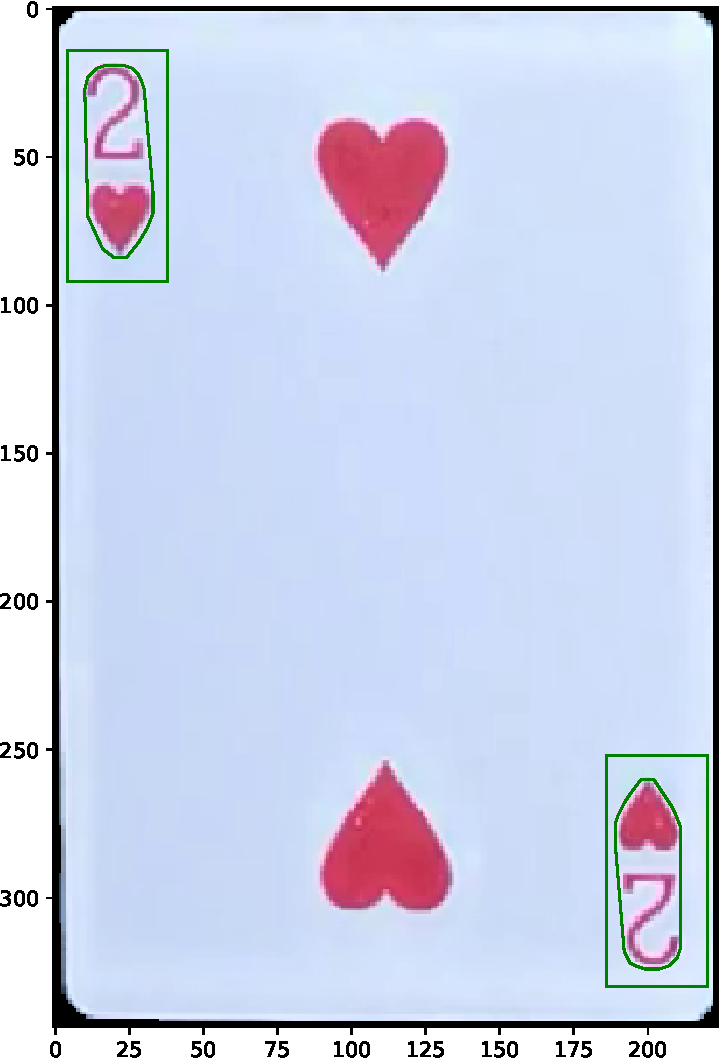
\includegraphics[scale=0.28]{slike/kartaHull.pdf}
 \end{figure}
\end{frame}
%%%%%%%%%%%%%%%%%%%%
\subsection{Прављење скупа за тренирање}
\begin{frame}
\frametitle{Прављење скупа за тренирање}
\begin{itemize}
 \item Скуп за тренирање се генерише подвлачењем једне од много позадина испод карата,
а оне се распоређују на два начина:
 \begin{itemize}
  \item Насумичним транслирањем, ротацијом и увећавањем
  \mbox{\alert{две карте}}
  \item  Извшавањем трансформација за две карте, а
  потом трансформацијом све \alert{три карте} карте као групе,
  после чега се налазе једна до друге као када се држе у руци
 \end{itemize}
\end{itemize}
\begin{figure}[H]
  \centering
      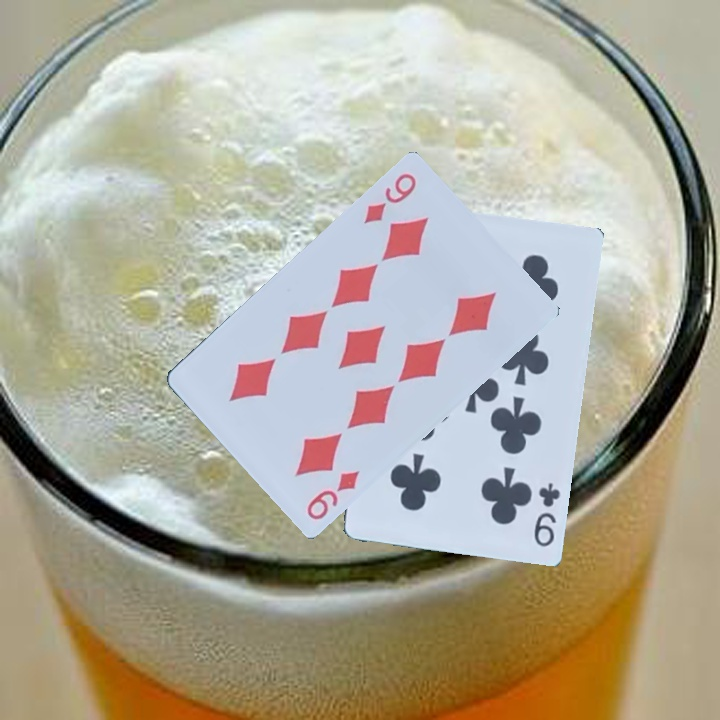
\includegraphics[scale=0.18]{slike/dveKarte.jpg} \hspace{1.2cm}
      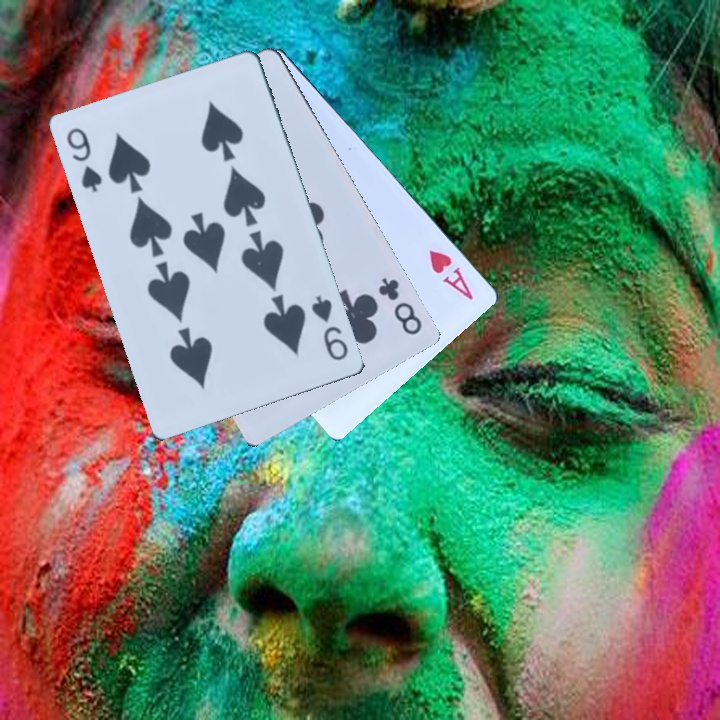
\includegraphics[scale=0.18]{slike/triKarte.jpg}
 \end{figure}
\end{frame}

%%%%%%%%%%%%%%%%%%%%%%%%%%%%%%%%%%%%%%%%%%%%%%%%%%%%%%
\section{Вештачке неуронске мреже - теорија}
%%%%%%%%%%%%%%%%%%%%
\subsection{Увод у вештачке неуронске мреже}
\begin{frame}
\frametitle{Увод у вештачке неуронске мреже}
\begin{itemize}
 \item \alert{Неурон} је основна јединица вештачке неуронске мреже и има своје улазе,
над којима извршава рачунске операције и добијену вредност уписује
као излаз
\begin{figure}[H]
  \centering
      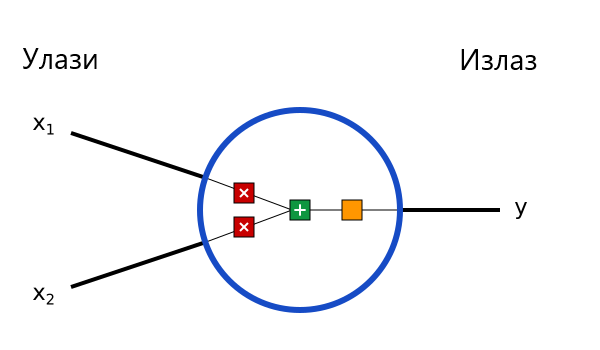
\includegraphics[scale=0.26]{slike/neuron.png} \hspace{1.2cm}      
      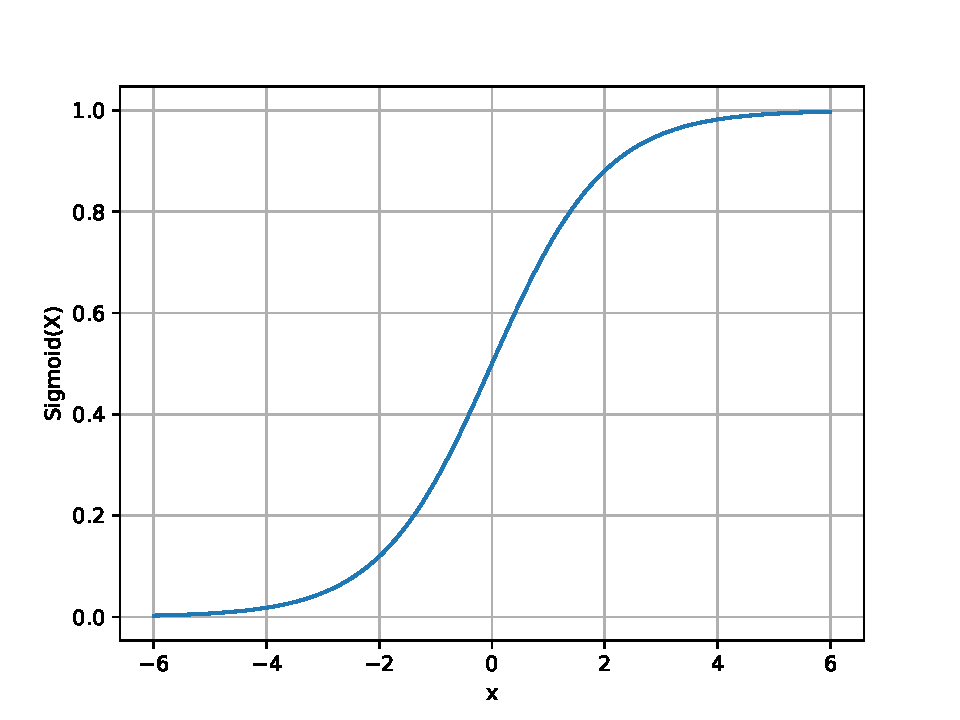
\includegraphics[scale=0.26]{slike/sigmoid}
 \end{figure}
 \item Формула за израчунавање вредности излаза
 је $y = f(x_1 * w_1 + x_2 * w_2 + b)$, где је $f$ \alert{активациона
 функција} (нпр. Сигмоидна функција, дефинисана као
 $S(x) = \frac{1}{1+e^{-x}}$)
 \item Процес прослеђивања улазних вредност напред назива се \alert{пропагација унапред}
\end{itemize}
\end{frame}

\begin{frame}
\frametitle{Увод у вештачке неуронске мреже}
\begin{itemize}
 \item \alert{Неуронска мрежа} је скуп међусобно повезаних неурона
 \begin{figure}[H]
  \centering
      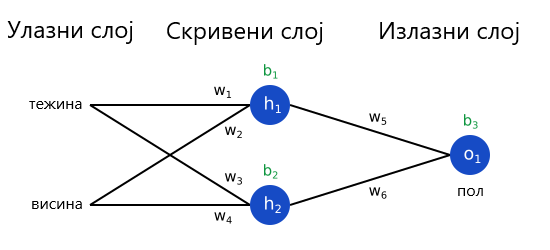
\includegraphics[scale=0.35]{slike/neuronskaMrezaOznake.png}
 \end{figure}
 \item \alert{Функцијa губитка} $L$ и \alert{функцијa трошка} $J$
 \item \alert{Тренирање} мреже je поступак промене вредности тежине веза и
прагова активације са циљем да се одреди \alert{што нижа функција трошка}
 \item На пример, функција трошка може бити \alert{\textit{средња квадратна грешка}}
 (\textit{mean square error}) и дефинише се као:
 \begin{equation}
 J = MSE = \frac{1}{m} \sum_{i=1}^{m} (y_{true} - y_{pred})^2
 \end{equation}
\end{itemize}
\end{frame}

\begin{frame}
\frametitle{Увод у вештачке неуронске мреже}
\begin{itemize}
 \item Функција трошка може да се представи као функција 
 са више променљивих:
 $Ј(w_1,w_2,w_3,w_4,w_5,w_6,b_1,b_2,b_3)$
 \item Промена вредности $w_1$, мења вредност $Ј$, па је потребно израчунати
 парцијални извод и своди се на чланове које је могуће израчунати и
 добија се:
 \begin{equation}
 \frac{\partial J}{\partial w_1} = \frac{\partial J}{\partial y_{pred}} * \frac{\partial y_{pred}}{\partial h_1} * \frac{\partial h_1}{\partial w_1}
 \end{equation}
 \item Поступак рачунања парцијалних извода идући од излаза ка улазу
  неуронске мреже
  назива се \alert{пропагација уназад}
 \item Алгоритам \alert{Стохастички градијентни спуст} би могао да се
 употреби за минимизовање функције трошка $J$:
 \begin{equation}
  w_1 \leftarrow w_1 - \eta \frac{\partial J}{\partial w_1}
 \end{equation}
 \begin{itemize}
  \item $\eta$ - \alert{дужинa корака при учењу} (\alert{learning rate})
 \end{itemize}
\end{itemize}
\end{frame}
%%%%%%%%%%%%%%%%%%%%
\subsection{Конволуцијске неуронске мреже}
\begin{frame}
\frametitle{Конволуцијске неуронске мреже}

\begin{itemize}
 \item \alert{Рачунарски вид} (\alert{Computer vision})
 \begin{itemize}
  \item Аутономна вожња, препознавање лица\dots
 \end{itemize}
 \item Проблем - \alert{слике} (подаци) на улазу могу да буду \alert{великe}
 \begin{itemize}
 \item Нека је слика на улазу димензија $1000 \times 1000 \times 3$,
 а први слој мреже има $1000$ неурона, тада би матрица
 тежина веза између прва два слоја имала димензије (1000,3000000) и
 \alert{израчунавање} постаје \alert{неизводљиво}
 \end{itemize}
\end{itemize}
\begin{figure}[H]
  \centering
      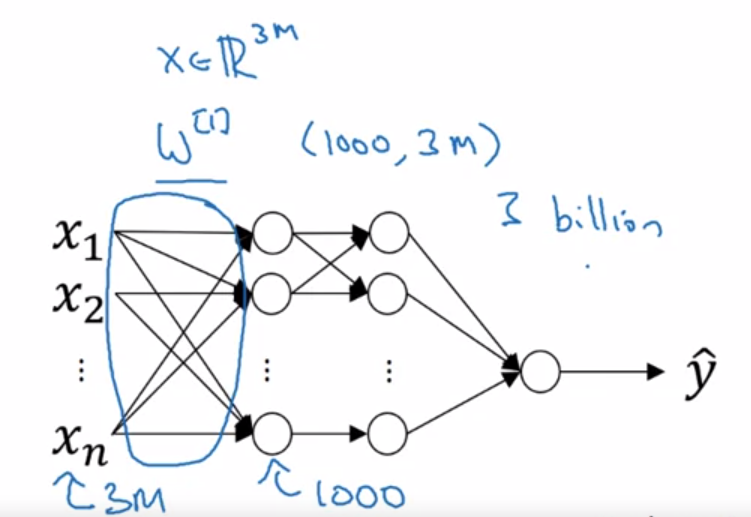
\includegraphics[scale=0.27]{slike/ngFCVision.png} \hspace{1.2cm}      
      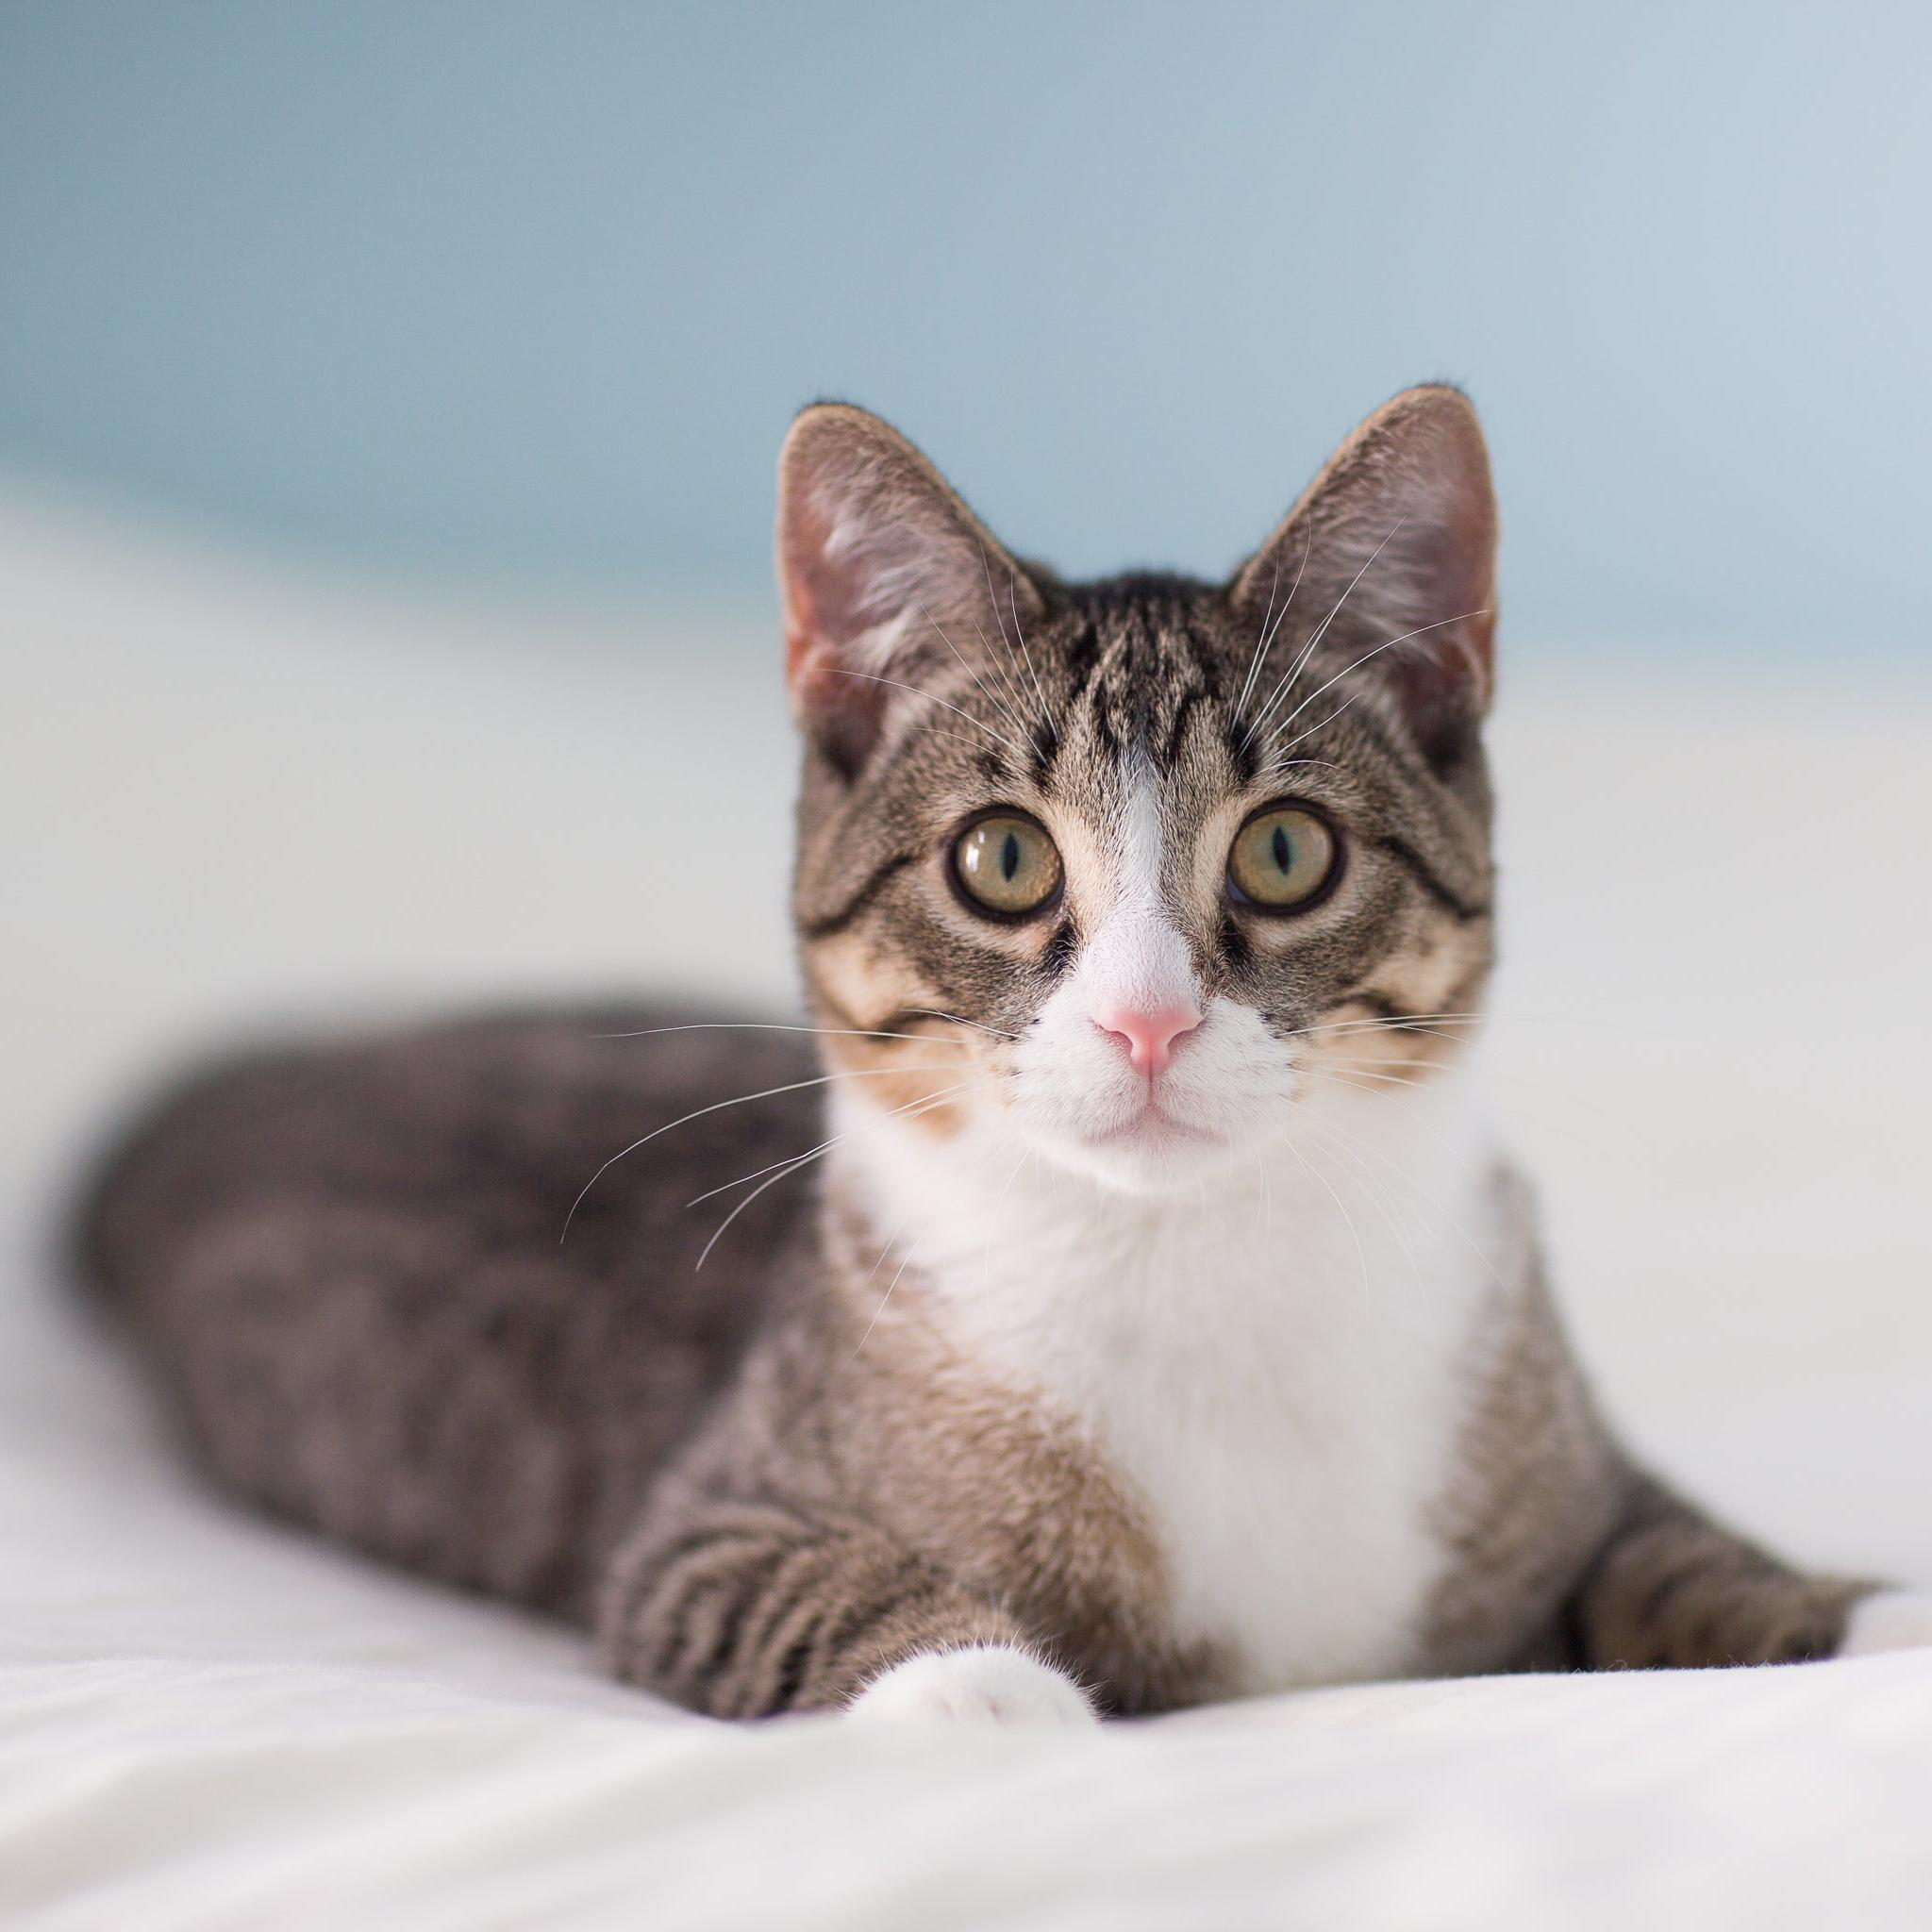
\includegraphics[scale=0.07]{slike/macka}
 \end{figure}
\end{frame}

\begin{frame}
\frametitle{Конволуцијске неуронске мреже}
\begin{itemize}
 \item Операција \alert{конволуције} је једна од основа за прављење конволуцијске
 неуронске мреже.
 \item Вредност поља (1,1) у излазној матрици једнака је збиру производа
 чланова исечка (димензија филтера), улазне матрице и чланова филтера. Исечак
 се помера у страну (следећи ред) и извршава се исти поступак.
\end{itemize}
\begin{figure}[H]
  \centering
      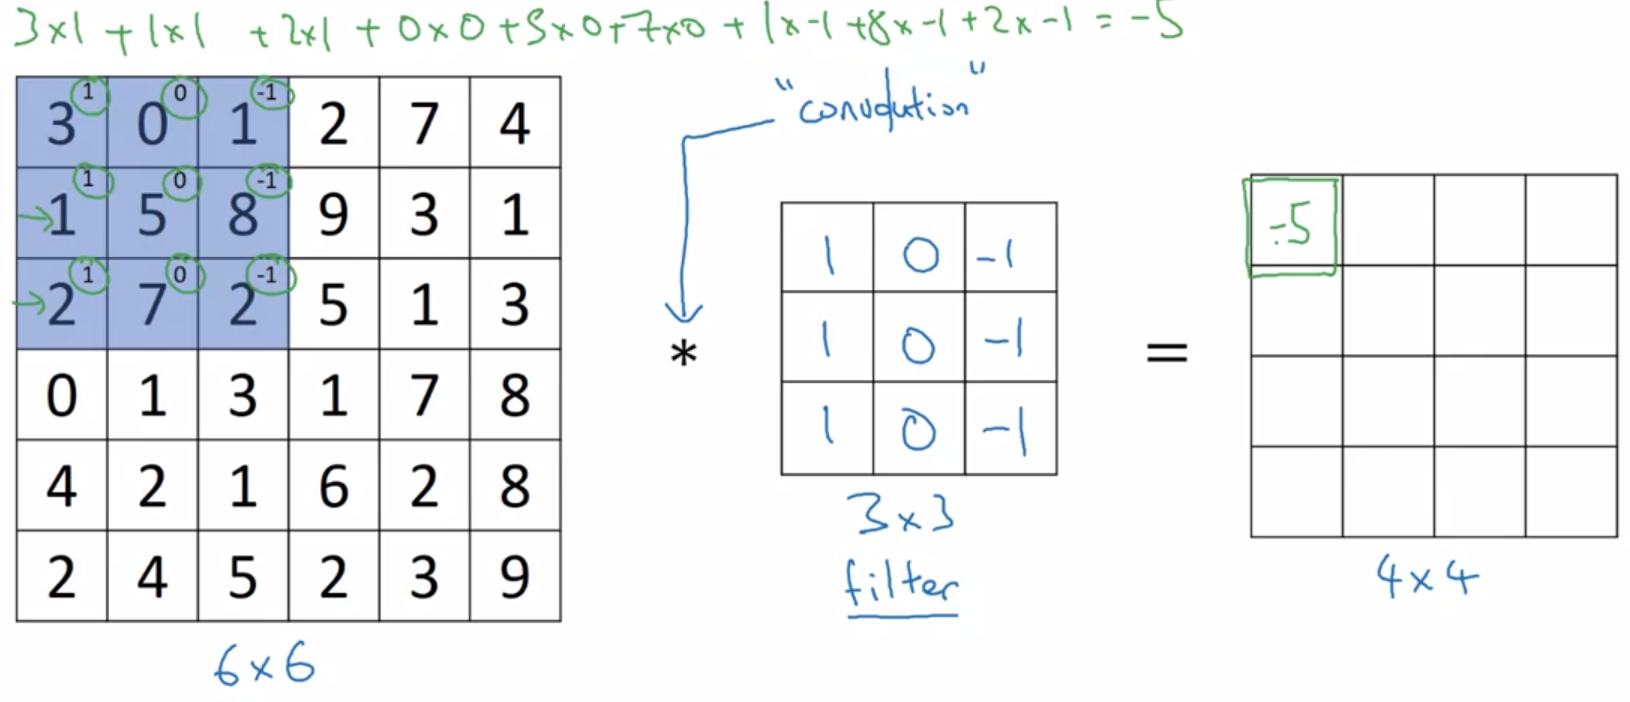
\includegraphics[scale=0.22]{slike/ngKonvoucija.png}
 \end{figure}
\end{frame}

\begin{frame}
\frametitle{Конволуцијске неуронске мреже}
\begin{itemize}
 \item Први корак при детекцији лица је \alert{детектовање ивица}
 \begin{figure}[H]
  \centering
      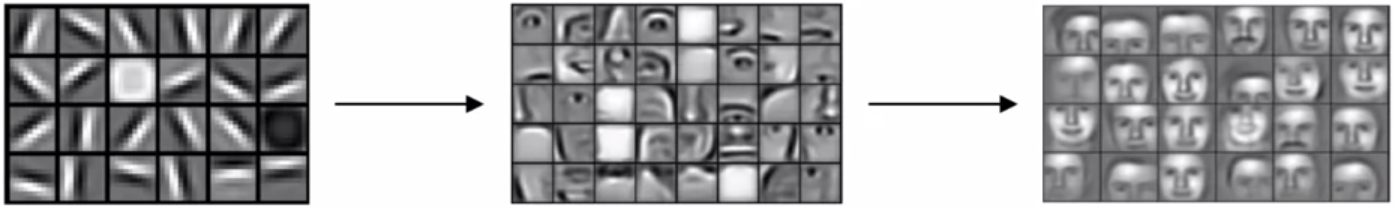
\includegraphics[scale=0.2]{slike/ngEdge1.png}
 \end{figure}
 \item Детектовање \alert{вертикалних} ивица
 \begin{itemize}
  \item Прелаз \alert{светло-у-тамно}
 \end{itemize}

 \begin{figure}[H]
  \centering
      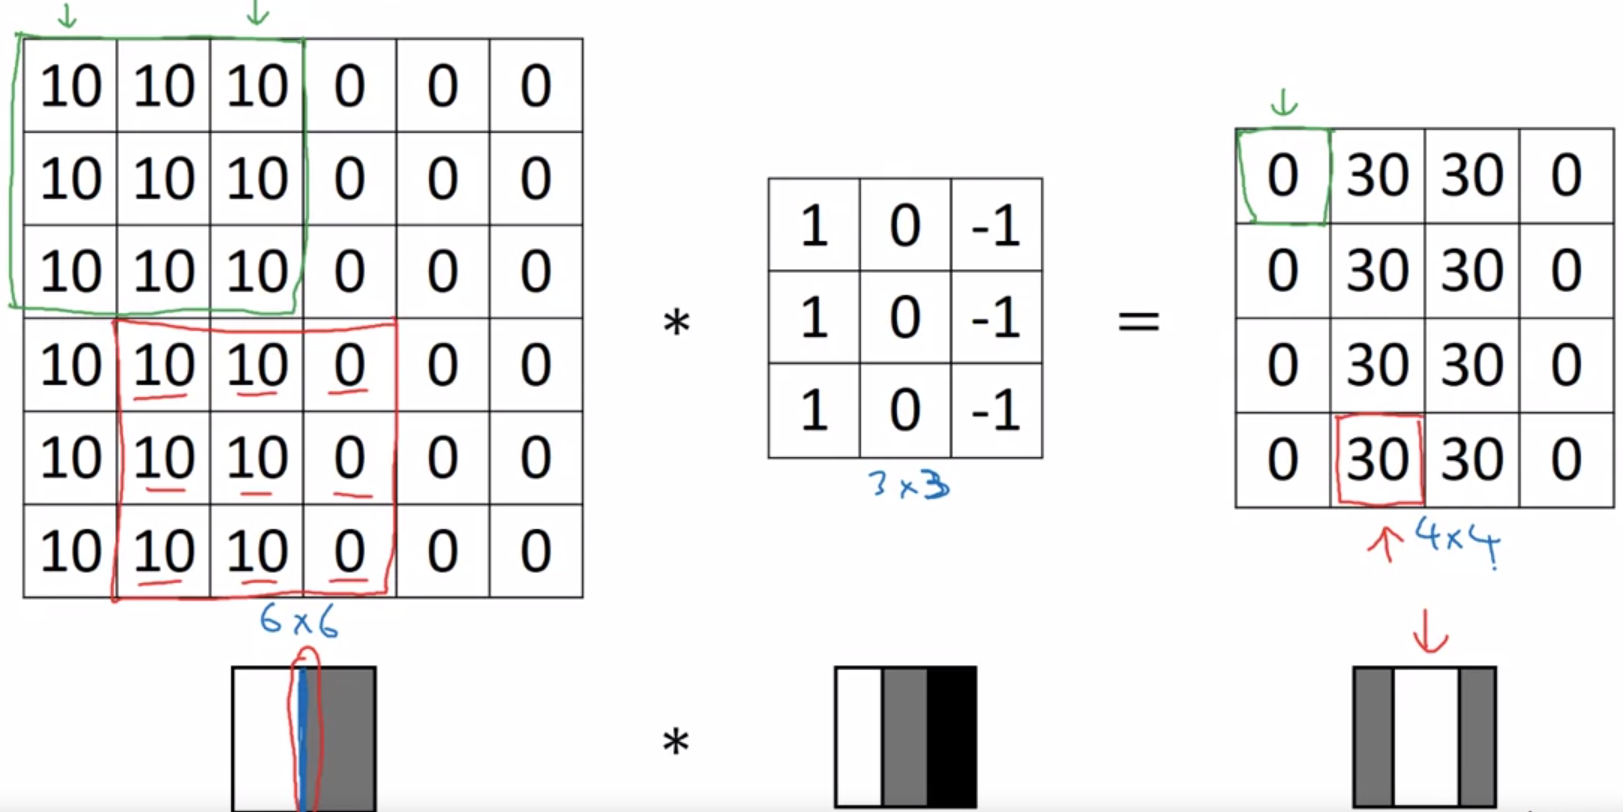
\includegraphics[scale=0.22]{slike/ngKonvoucijaVert.png}
 \end{figure}
\end{itemize}
\end{frame}

\begin{frame}
\frametitle{Конволуцијске неуронске мреже} 
\begin{itemize}
 \item С обзиром да постоји \alert{много различитих ивица},
  а њихова детекција се врши
  применом различитих филтера тј. вредности 
  \alert{поља матрице филтера} су различите,
  могуће их је посматрати као \alert{параметре} за \alert{тренирање}
 \item \alert{Допуњавање матрице} (\alert{padding})
  \begin{itemize}
  \item мање информација које се односе на средину матрице
  \item чување информацијa из поља са ивице слике
  \end{itemize}
\end{itemize}
\begin{equation}
  \begin{bmatrix}
  w_1 & w_2 & w_3 \\
  w_4 & w_5 & w_6 \\
  w_7 & w_8 & w_9
  \end{bmatrix}
  \begin{bmatrix}
  0 & 0 & 0 & 0 & 0 & 0 & 0 \\
  0 &   &   &   &   &   & 0 \\
  0 &   &   &   &   &   & 0 \\
  0 &   &   &   &   &   & 0 \\
  0 &   &   &   &   &   & 0 \\
  0 &   &   &   &   &   & 0 \\
  0 & 0 & 0 & 0 & 0 & 0 & 0
  \end{bmatrix}
  \end{equation}
\end{frame}

\begin{frame}
\frametitle{Конволуцијске неуронске мреже}
\begin{itemize}
 \item \alert{Конволуција са већим кораком} (\alert{Strided convolution})
  се разликује у \alert{кораку} (\alert{stride}) који исечак прави
  кроз улазну матрицу.
  \begin{figure}[H]
    \centering
	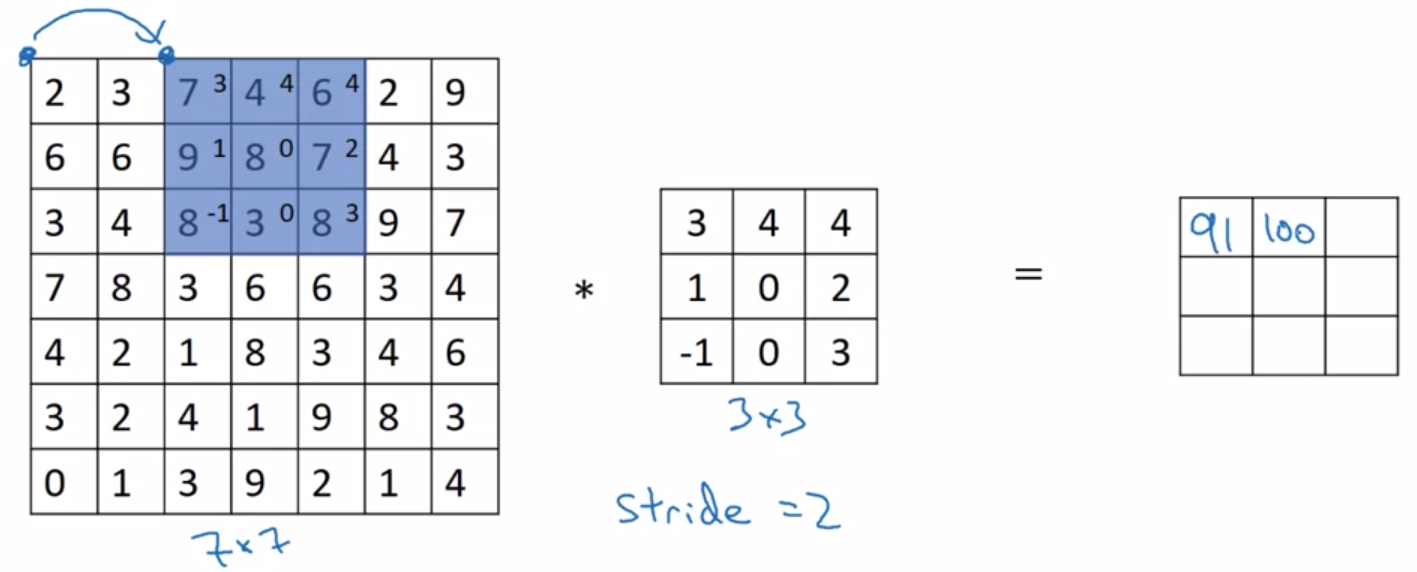
\includegraphics[scale=0.22]{slike/ngConvStride1.png}
  \end{figure}
 \item Нека је слика димензија $n \times n$, а филтер $f \times f$,
 \textit{корак} je $s$, а
 \textit{допуна} $p$,
  тада је \alert{димензија излазне матрице}:
  \begin{equation*}
  \floor*{\frac{n+2p-f}{s}+1} \times \floor*{\frac{n+2p-f}{s}+1}
  \end{equation*}
\end{itemize}
\end{frame}

\begin{frame}
\frametitle{Конволуцијске неуронске мреже}
\begin{itemize}
 \item Пример једног слоја конволуцијске неуронске мреже
 \item \alert{Kолико год да је слика велика,
  број параметара за тренирање је дефинисан димензијама филтера!}
\end{itemize}
\begin{figure}[H]
    \centering
	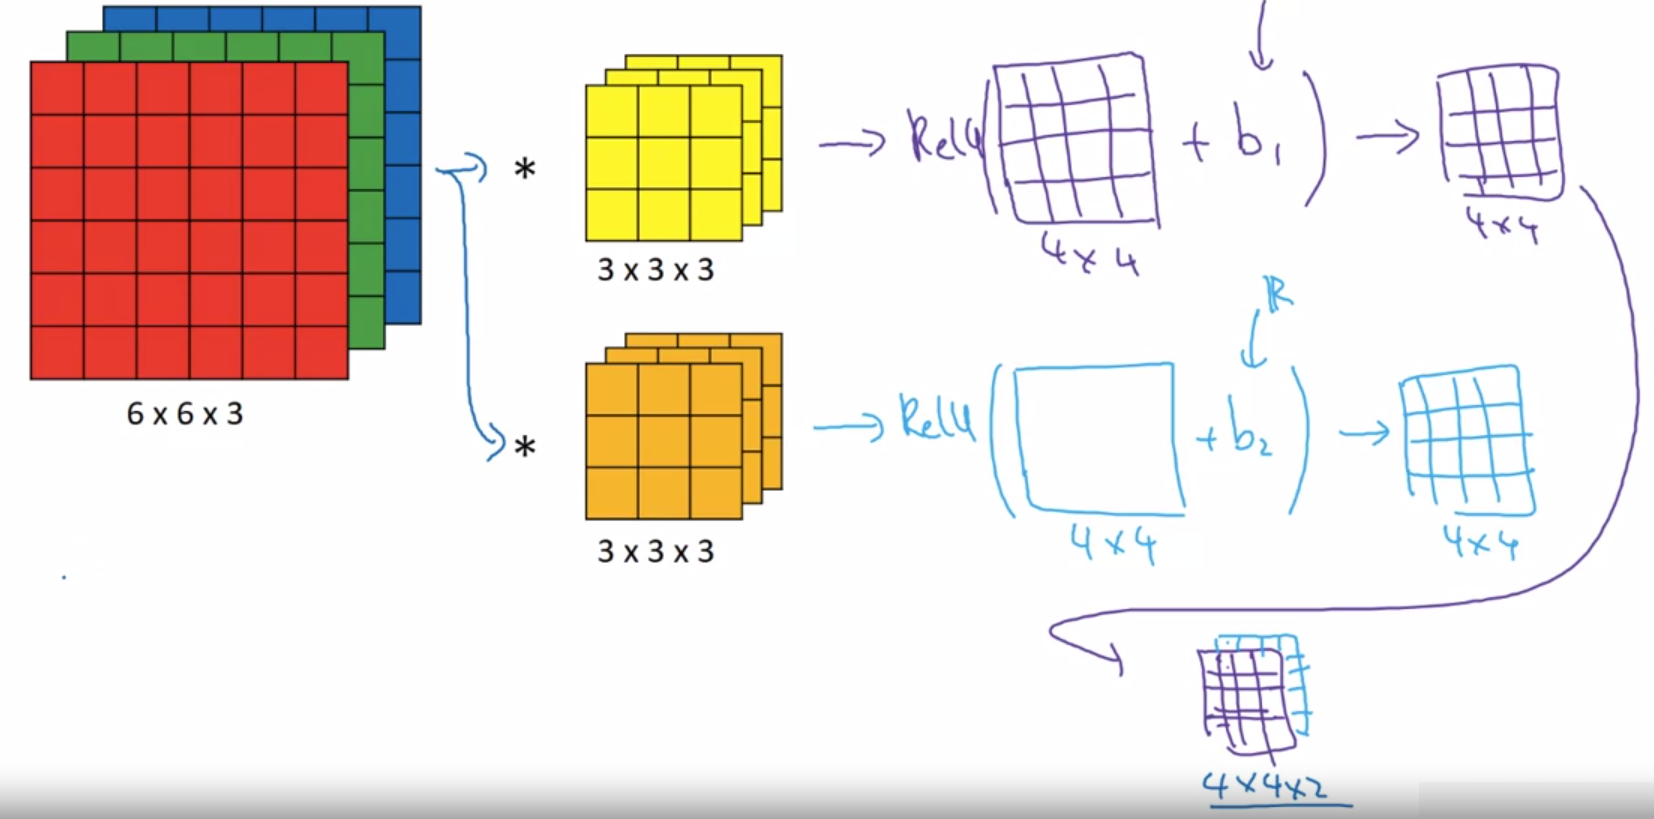
\includegraphics[scale=0.22]{slike/ngConvLay1.png}
  \end{figure}
\end{frame}

\begin{frame}
\frametitle{Конволуцијске неуронске мреже}
\begin{itemize}
 \item Врло често је матрица на излазу веома велика и можда ју је потребно
  смањити, а да притом главне \textit{одлике} буду сачуване.
  Ово се постиже \textbf{Слојевима удруживања} (\textbf{Pooling layers}) и
  слика приказује један тип који се назива
  \alert{Удруживање максимума} (\alert{Max pooling}).
 \item Максимална
  вредност у исечку се уписује као излазна
  \begin{itemize}
   \item већа вредност од осталих у исечку представља
   \textit{одлику} и остаје сачувана
   \item уколико су вредности приближне, уписана вредност
   је само мало већа
  \end{itemize}

\end{itemize}
\begin{figure}[H]
  \centering
      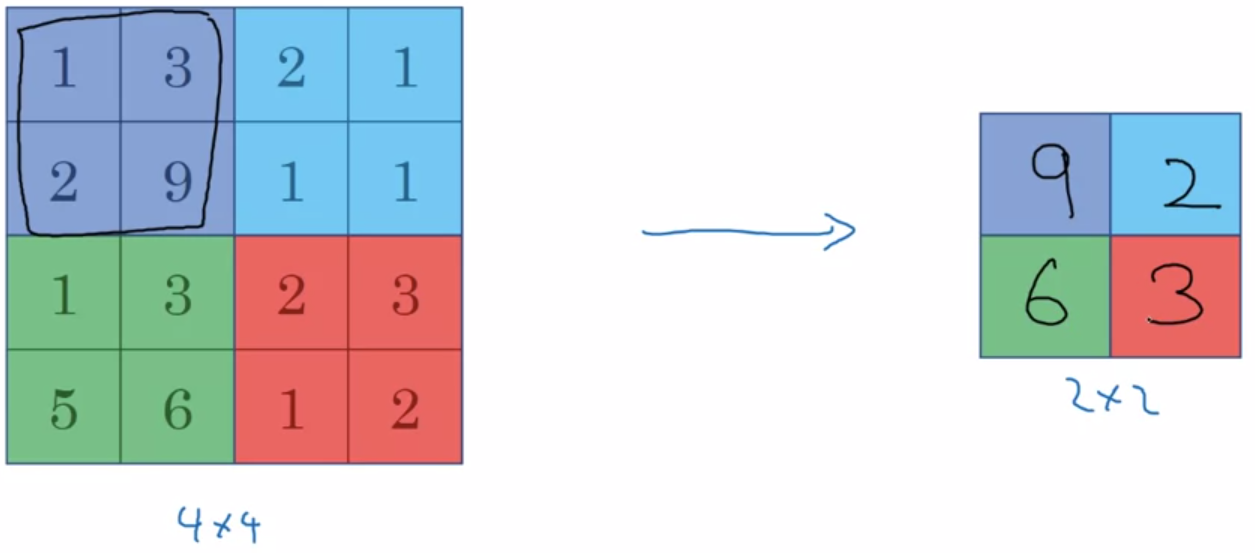
\includegraphics[scale=0.18]{slike/ngMaxPool.png}
  \label{fig:ng_MaxPool}
\end{figure}
\end{frame}

\begin{frame}
\frametitle{Конволуцијске неуронске мреже}
\begin{itemize}
 \item Две \alert{предности коришћења конволуцијских неуронских мрежа} су:
 \begin{itemize}
  \item \alert{Дељење параметара}: филтер који детектује одређене \textit{ивице}
 у једном делу слике, врло вероватно ће подједнако добро радити
 и у другом делу слике.
 
 \item \alert{Ређе зависности} (\alert{Sparsity of connections}):
 У сваком слоју, ниједна излазна вредност не зависи од много улазних.
 Свако поље матрице на излазу је
 израчунато из малог исечка слике са улаза и не зависи од осталих.
 \end{itemize}
 \item Конволуцијске неуронске мреже, овим одликамa,
 омогућавају \alert{тренирање над мањим скуповима} и 
  \alert{теже долази до претренирања} (\alert{overfitting}).
\end{itemize}
\end{frame}
%%%%%%%%%%%%%%%%%%%%
\subsection{YOLO алгоритам}
\begin{frame}
\frametitle{YOLO алгоритам}
\begin{itemize}
 \item \alert{Класификација} слике је одређивање класе
објекта на слици, а \alert{локализација} објекта је његово означавање
 \item \alert{Детекција} објеката је проблем када се на слици
 налази више објеката које треба класификовати и локализовати
 \item Претпоставимо да детектујемо три класе: 1.\ пешак, 2.\ аутомобил,
 3.\ мотоцикл
\end{itemize}
  \begin{figure}[H]
    \centering
	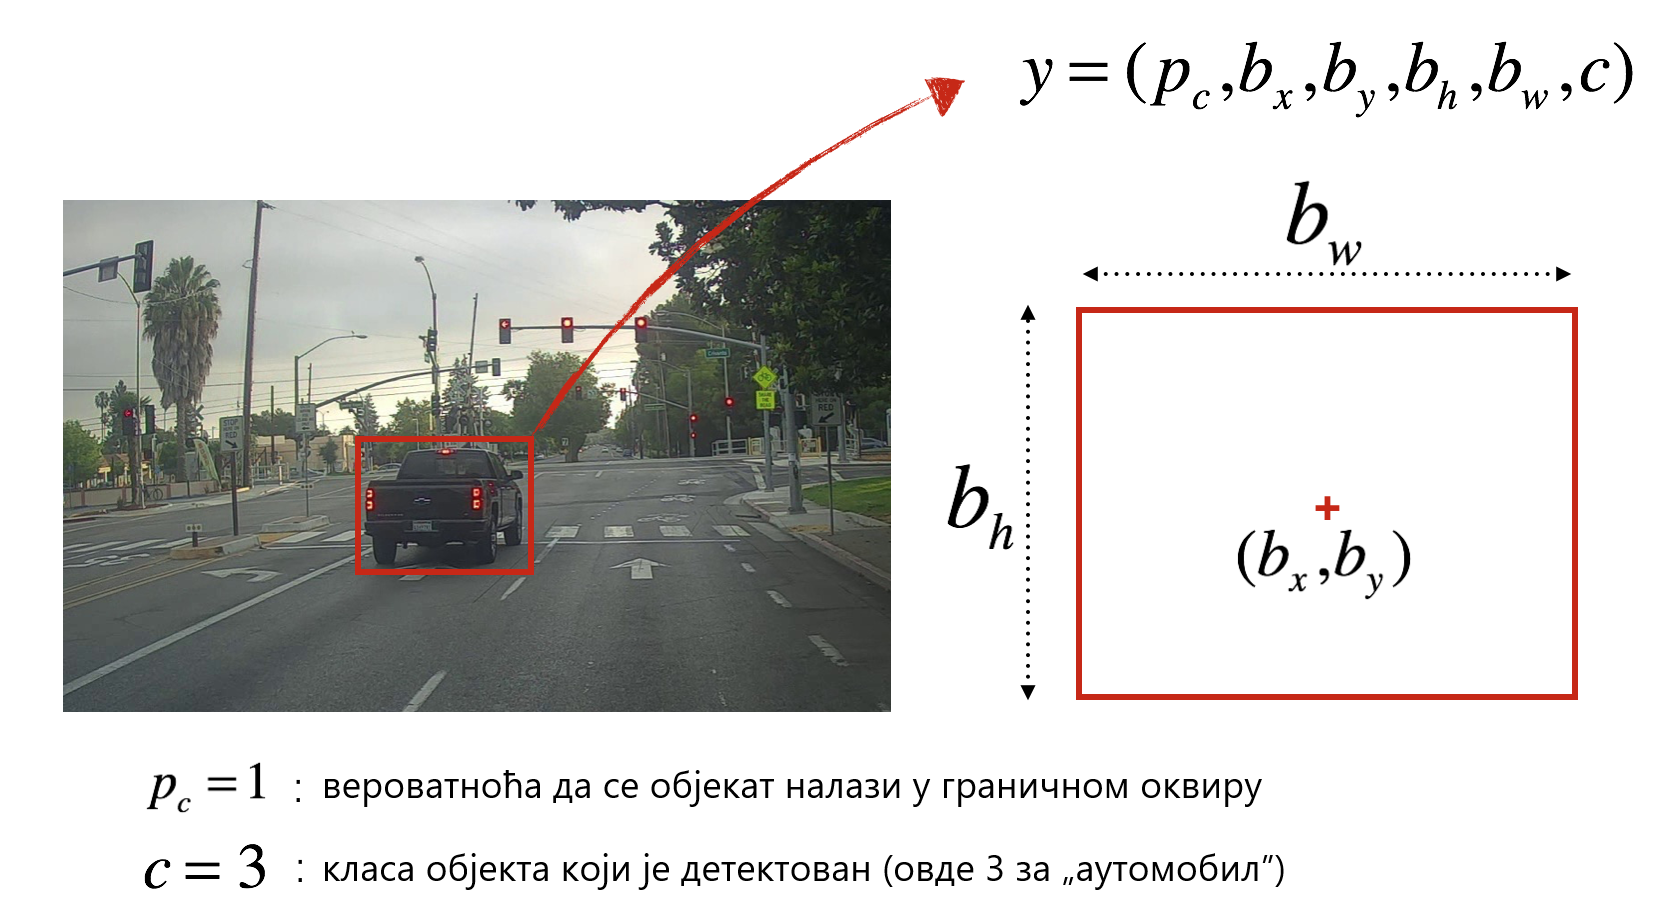
\includegraphics[scale=0.18]{slike/box_label.png}
  \end{figure}
\end{frame}

\begin{frame}
\frametitle{YOLO алгоритам}
\begin{itemize}
  \item Параметар \alert{$c$} може да буде или \alert{целобројна}
  вредност која представља класу \alert{или
  вектор} димензија броја класа које детектујемо, где члан вектора који
  представља класу има вредност $1$, а остали имају вредност нула.
  \item Ako нема објеката, вероватноћа $p_c$ ће бити
  0, па су остали чланови вектора небитни
\end{itemize}
 \begin{equation}
  y =
  \begin{bmatrix}
  p_c \\
  b_x \\
  b_y \\
  b_h \\
  b_w \\
  c_1 \\
  c_2 \\
  c_3
  \end{bmatrix}
  =
  \begin{bmatrix}
  1 \\
  b_x \\
  b_y \\
  b_h \\
  b_w \\
  0 \\
  1 \\
  0
  \end{bmatrix} \qquad
  y =
  \begin{bmatrix}
  p_c \\
  b_x \\
  b_y \\
  b_h \\
  b_w \\
  c_1 \\
  c_2 \\
  c_3
  \end{bmatrix}
  =
  \begin{bmatrix}
  0 \\
  ? \\
  ? \\
  ? \\
  ? \\
  ? \\
  ? \\
  ?
  \end{bmatrix}
  \end{equation}
\end{frame}

\begin{frame}
\frametitle{YOLO алгоритам}
\begin{itemize}
 \item \alert{Детекцијa објеката клизним прозорима}
 \item Сваки \textbf{прозор} се \textbf{проследи конволуцијској мрежи},
 која даје резултат \textbf{да ли има објекта} у прослеђеном исечку слике
  или не. \alert{Прозор} треба да \alert{проклиза} кроз целу слику
  и овај поступак се може \alert{поновити и са већим прозором}
  \item Проблем оваквог приступа је \alert{превелико време извршавања}
\end{itemize}
\begin{figure}[H]
  \centering
      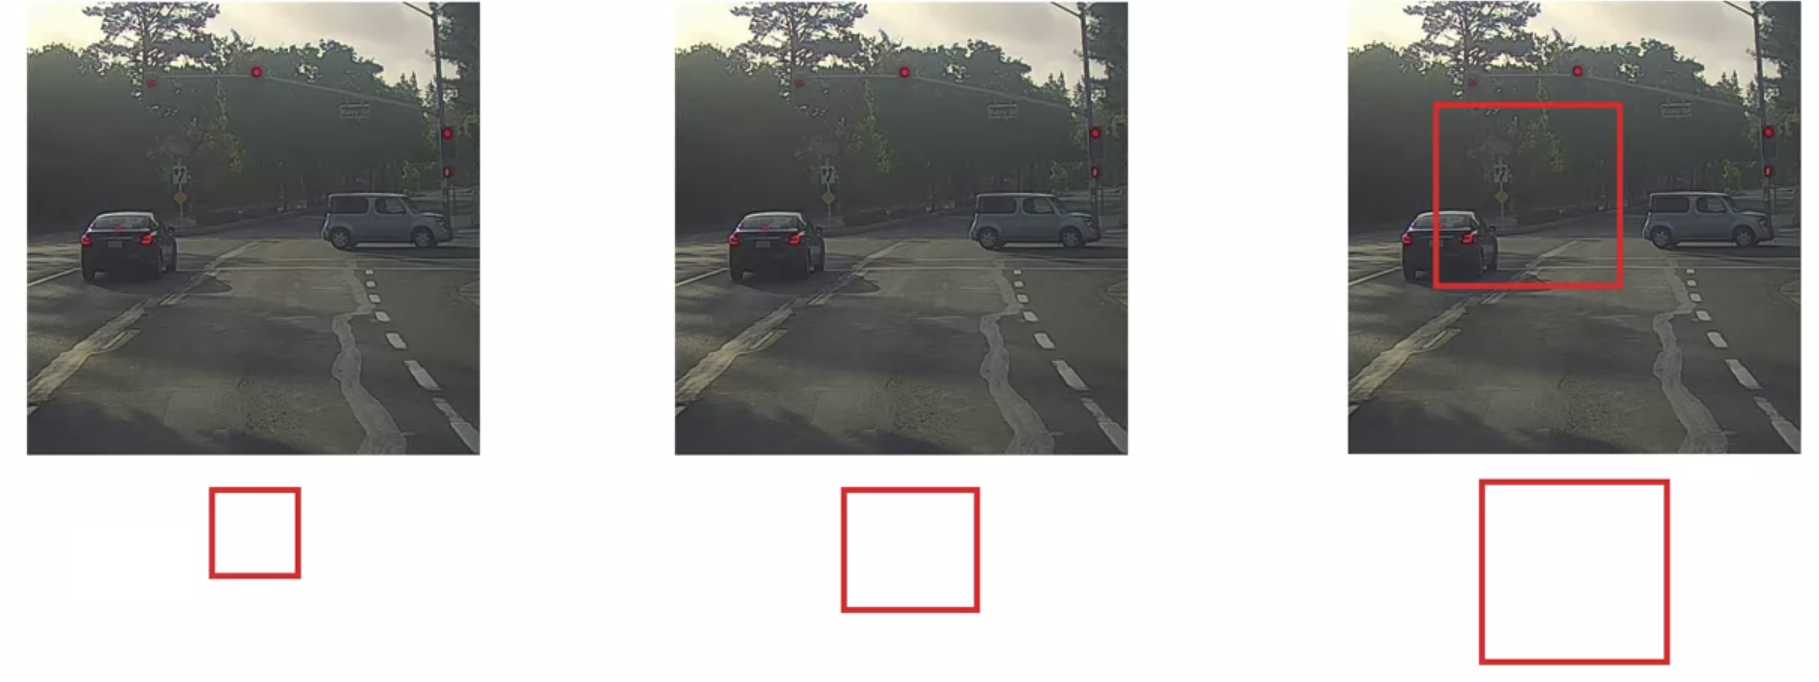
\includegraphics[scale=0.18]{slike/slidW.png}
\end{figure}
\end{frame}

\begin{frame}
\frametitle{YOLO алгоритам}
\begin{itemize}
 \item \alert{Конволуцијска имплементација је ефикаснија}
 \item Прва мрежа на крају
  садржи два \textit{потпуно повезана слоја} (\textit{fully connected layers}).
  Ова два слоја праве проблем тј.\ успоравају детекцију, јер је
  потребно посебно извршавање за сваки \textit{прозор} тј.\ исечак слике.
 \item У другом случају се примењују филтери \dots
\end{itemize}
\begin{figure}[H]
  \centering
      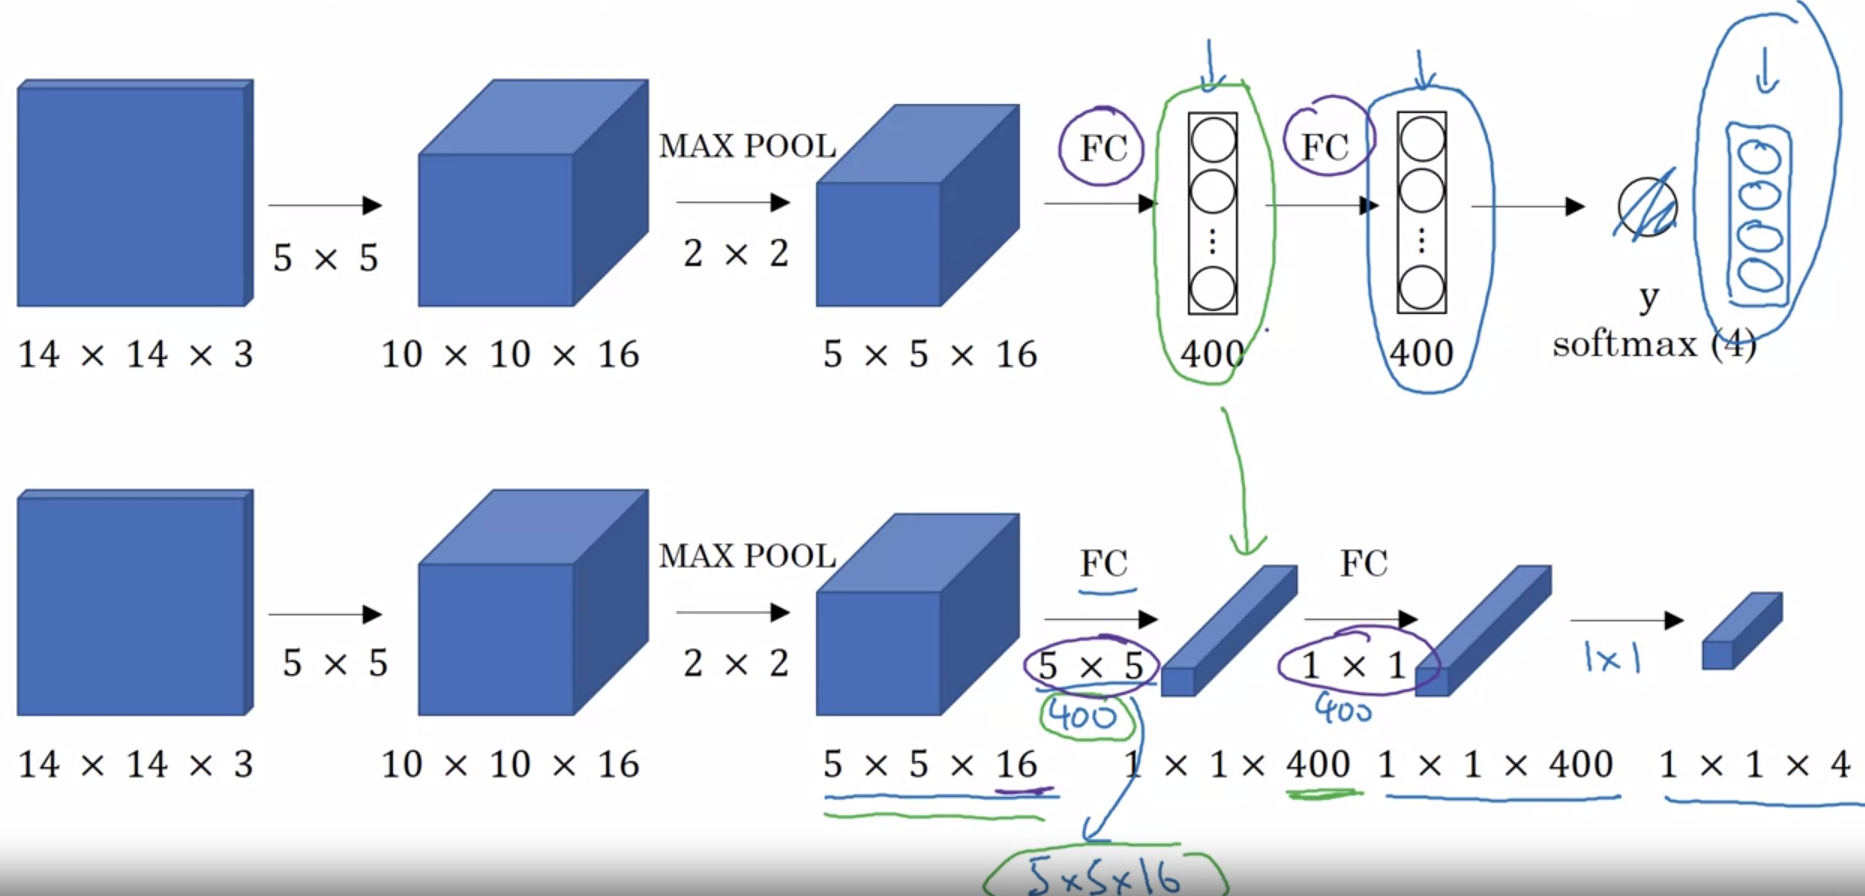
\includegraphics[scale=0.18]{slike/ngSlidWConv1.png}
\end{figure}
\end{frame}

\begin{frame}
\frametitle{YOLO алгоритам}
\begin{itemize}
 \item Случај када се на улазу нађе \alert{слика већих димензија}
\end{itemize}
\begin{figure}[H]
  \centering
      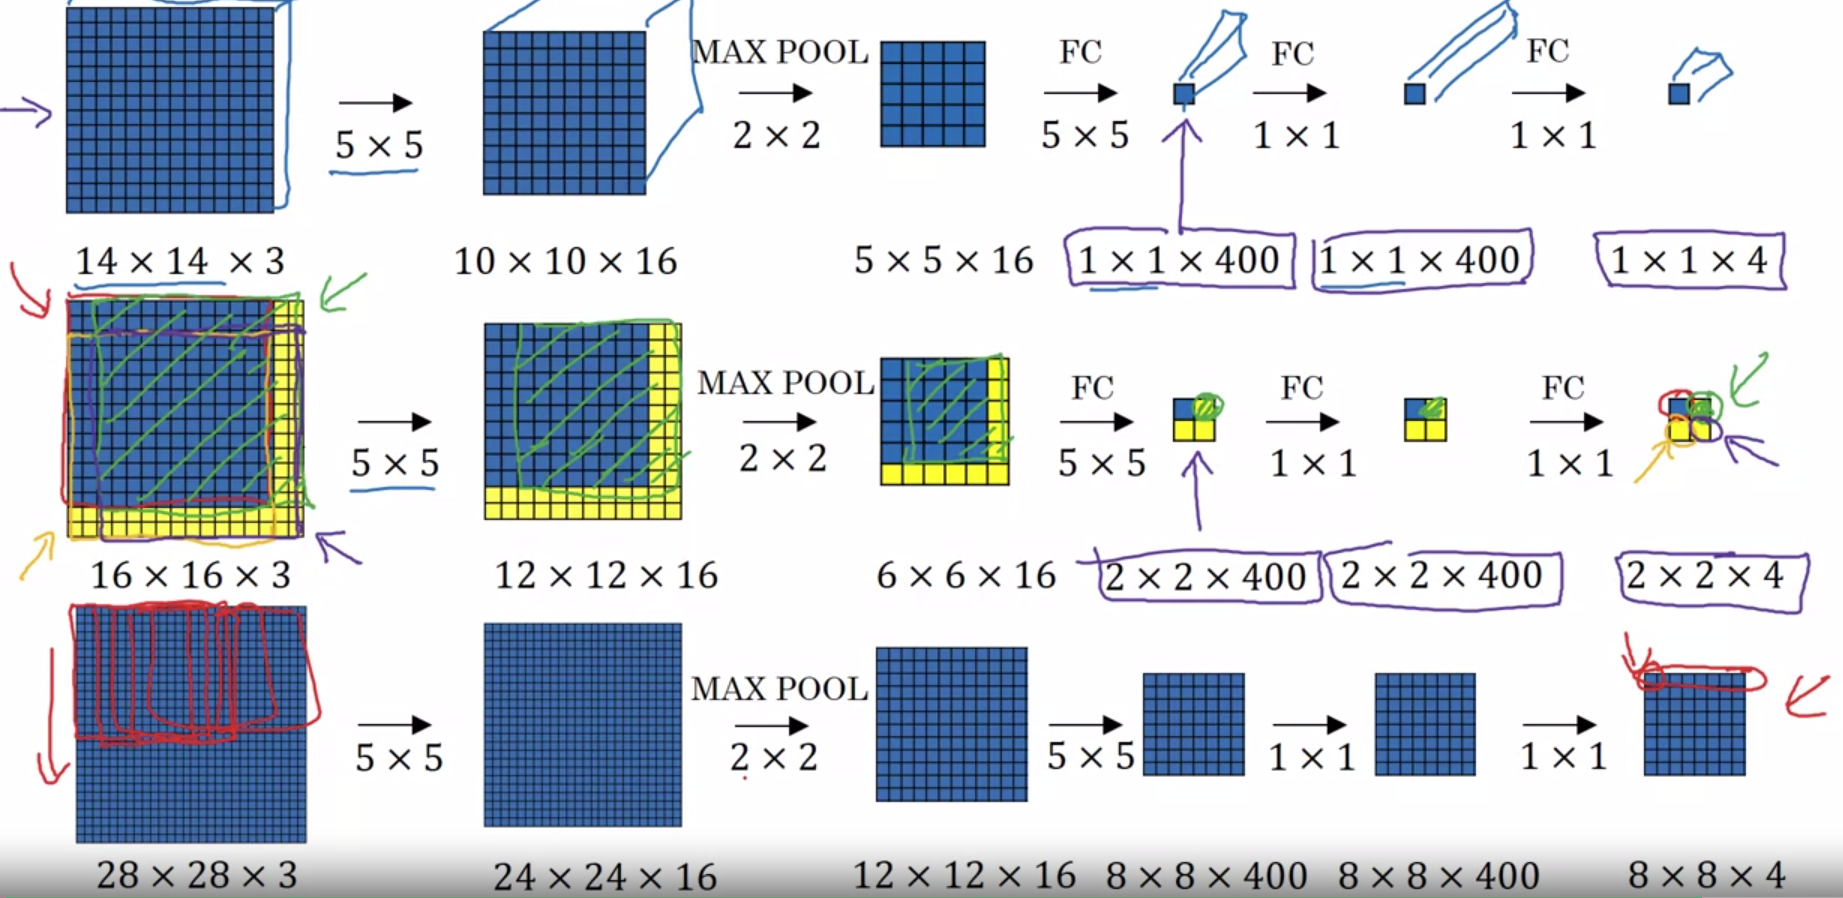
\includegraphics[scale=0.22]{slike/ngSlidWConv2.png}
\end{figure}
\end{frame}

\begin{frame}
\frametitle{YOLO алгоритам}
\begin{itemize}
 \item Вероватноће да се унутар квадрата налазе тражени објекти
 се добијају \alert{истовремено} за све исечке слике
 \item Потребно је изабрати најбољи гранични оквир, па се уводи
 \alert{ПпУ - Пресек преко Уније} (\alert{IoU - Intersection over Union}),
 дефинисан као $IoU = \frac{\textcolor{yellow}{\cap}}{\textcolor{green}{\cup}}$:
\end{itemize}
\begin{figure}[H]
  \centering
      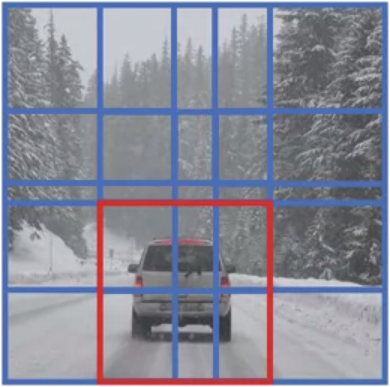
\includegraphics[scale=0.4]{slike/ngSlidWConv3.png} \qquad
      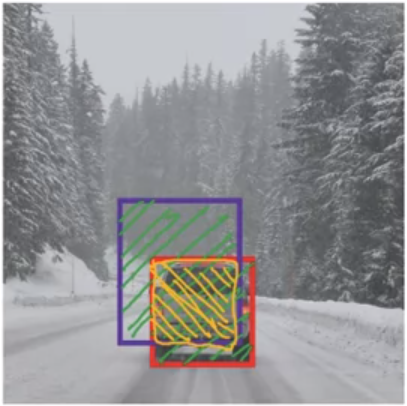
\includegraphics[scale=0.38]{slike/ngIoU.png}
\end{figure}
\end{frame}

\begin{frame}
\frametitle{YOLO алгоритам}
\begin{itemize}
 \item Поступак у коме се \alert{потискују} оквири који
 немају максималну вероватноћу детекције назива се
 \alert{Не-Масимално потискивање} (\alert{Non-Max suppression})
 \begin{figure}[H]
  \centering
      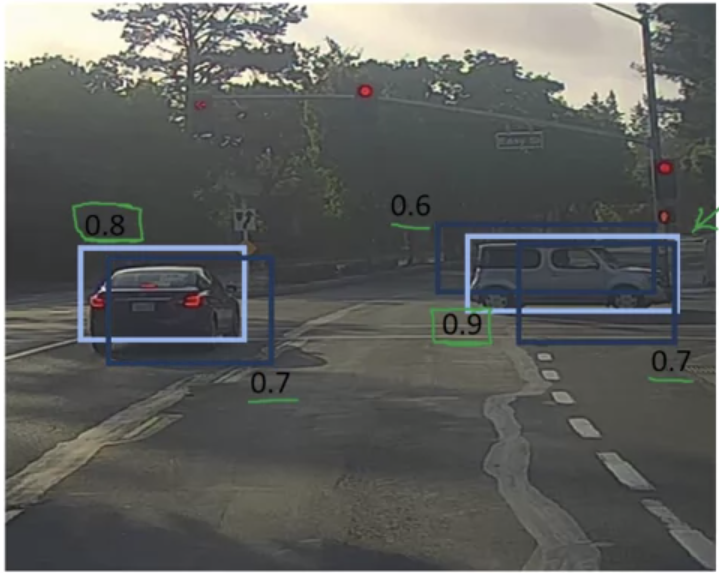
\includegraphics[scale=0.24]{slike/ngNonMax1.png}
\end{figure}
  \item Одбацити све оквире где је вероватноћа $p_c \leq 0.6$
  \item Док год има непроверених оквира:
    \begin{itemize}
    \item Изабрати оквир са највећом вероватноћом $p_c$
    \item Одбацити све преостале оквире где је $IoU \geq 0.5$ у односу на
    оквир из претходног корака
    \end{itemize}
  \end{itemize}
\end{frame}

\begin{frame}
\frametitle{YOLO алгоритам}
\begin{itemize}
 \item Слика се дели \alert{решетком} димензија $19 \times 19$, а
 објекат се \alert{додељује пољу} у коме се налази \alert{центар објекта}
 \item Могуће је да центри
 припадају \alert{истом пољу}, па се уводе \alert{класни оквири}
 (\alert{Anchor boxes})
 \item У случају детекције пешака и аутомобила,
 \alert{вектор} детекције је \alert{дупло већи} ($2 \times 8 = 16$)
 \item Објекат се додељује пару \alert{(пољеРешетке,класниОквир)}

\end{itemize}
\begin{figure}[H]
  \centering
      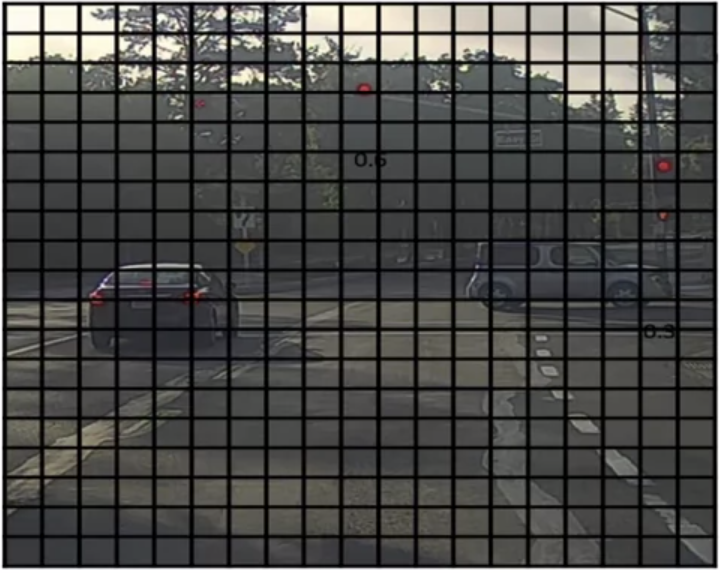
\includegraphics[scale=0.25]{slike/ngNonMax2.png} \qquad
      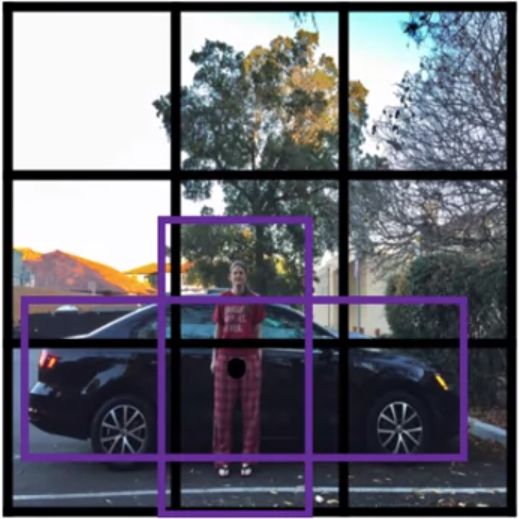
\includegraphics[scale=0.27]{slike/ngAnchor1.png}
\end{figure}
\end{frame}

\begin{frame}
\frametitle{YOLO алгоритам}
\begin{itemize}
 \item \alert{YOLO} (\alert{You Only Look Once}) \alert{алгоритам} на
 примеру детекције \textit{пешака} и \textit{аутомобила}:
 \begin{itemize}
  \item За сваку \textit{ћелију решетке} наћи 2 гранична
  оквира
  \item Занемарити оквире са малом вероватноћом детекције
  \item За сваку класу је потребно извршити Не-Масимално
  потискивање (Non-Max suppression)
 \end{itemize}
\end{itemize}
\begin{figure}[H]
  \centering
      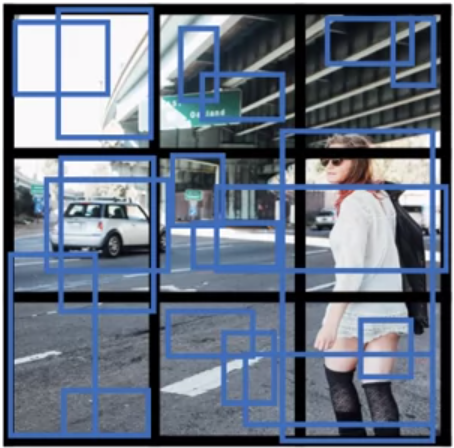
\includegraphics[scale=0.26]{slike/ngYOLO2.png} \quad
      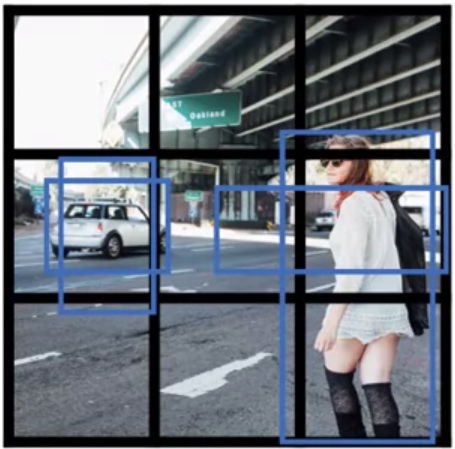
\includegraphics[scale=0.26]{slike/ngYOLO3.png} \quad
      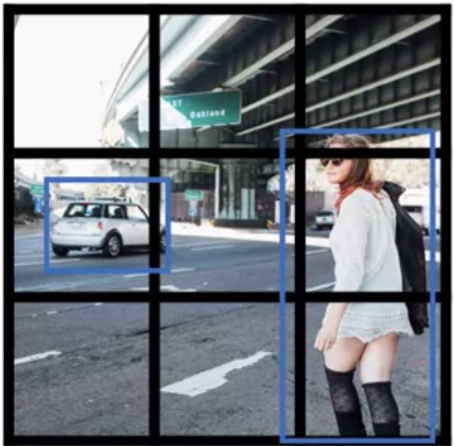
\includegraphics[scale=0.26]{slike/ngYOLO4.png}
\end{figure}
\end{frame}
%%%%%%%%%%%%%%%%%%%%%%%%%%%%%%%%%%%%%%%%%%%%%%%%%%%%%%
\section{Тренирање - Darknet програмски оквир}
\begin{frame}
\frametitle{Тренирање - Darknet програмски оквир}
\begin{itemize}
 \item Тренирање је извршено на \alert{GoogleColaboratory} виртуелној машини
 \item Пребацивање слика из GoogleDrive-а у виртуелну машину
 \item У датотеци \alert{yolov4-obj.cfg} се подешавају
 конфигурациони параметри:
 \begin{itemize}
  \item \alert{width}=416; \alert{height}=416; \alert{max\_batches}=104000;
 \alert{steps}=83200,93600; \alert{filters}=171
 \end{itemize}
 \item Тренирање почиње од иницијалних вредности тежина веза
  сачуваних у датотеци \alert{yolov4.conv.137}
\end{itemize}
\end{frame}

\begin{frame}
\frametitle{Тренирање - Darknet програмски оквир}
\begin{itemize}
 \item Параметар \alert{-thresh 0.8}  омогућава да се као
резултат прикажу само оне детекције где је верoватноћа $\geq 0.8$
\end{itemize}
\begin{figure}[H]
  \centering
      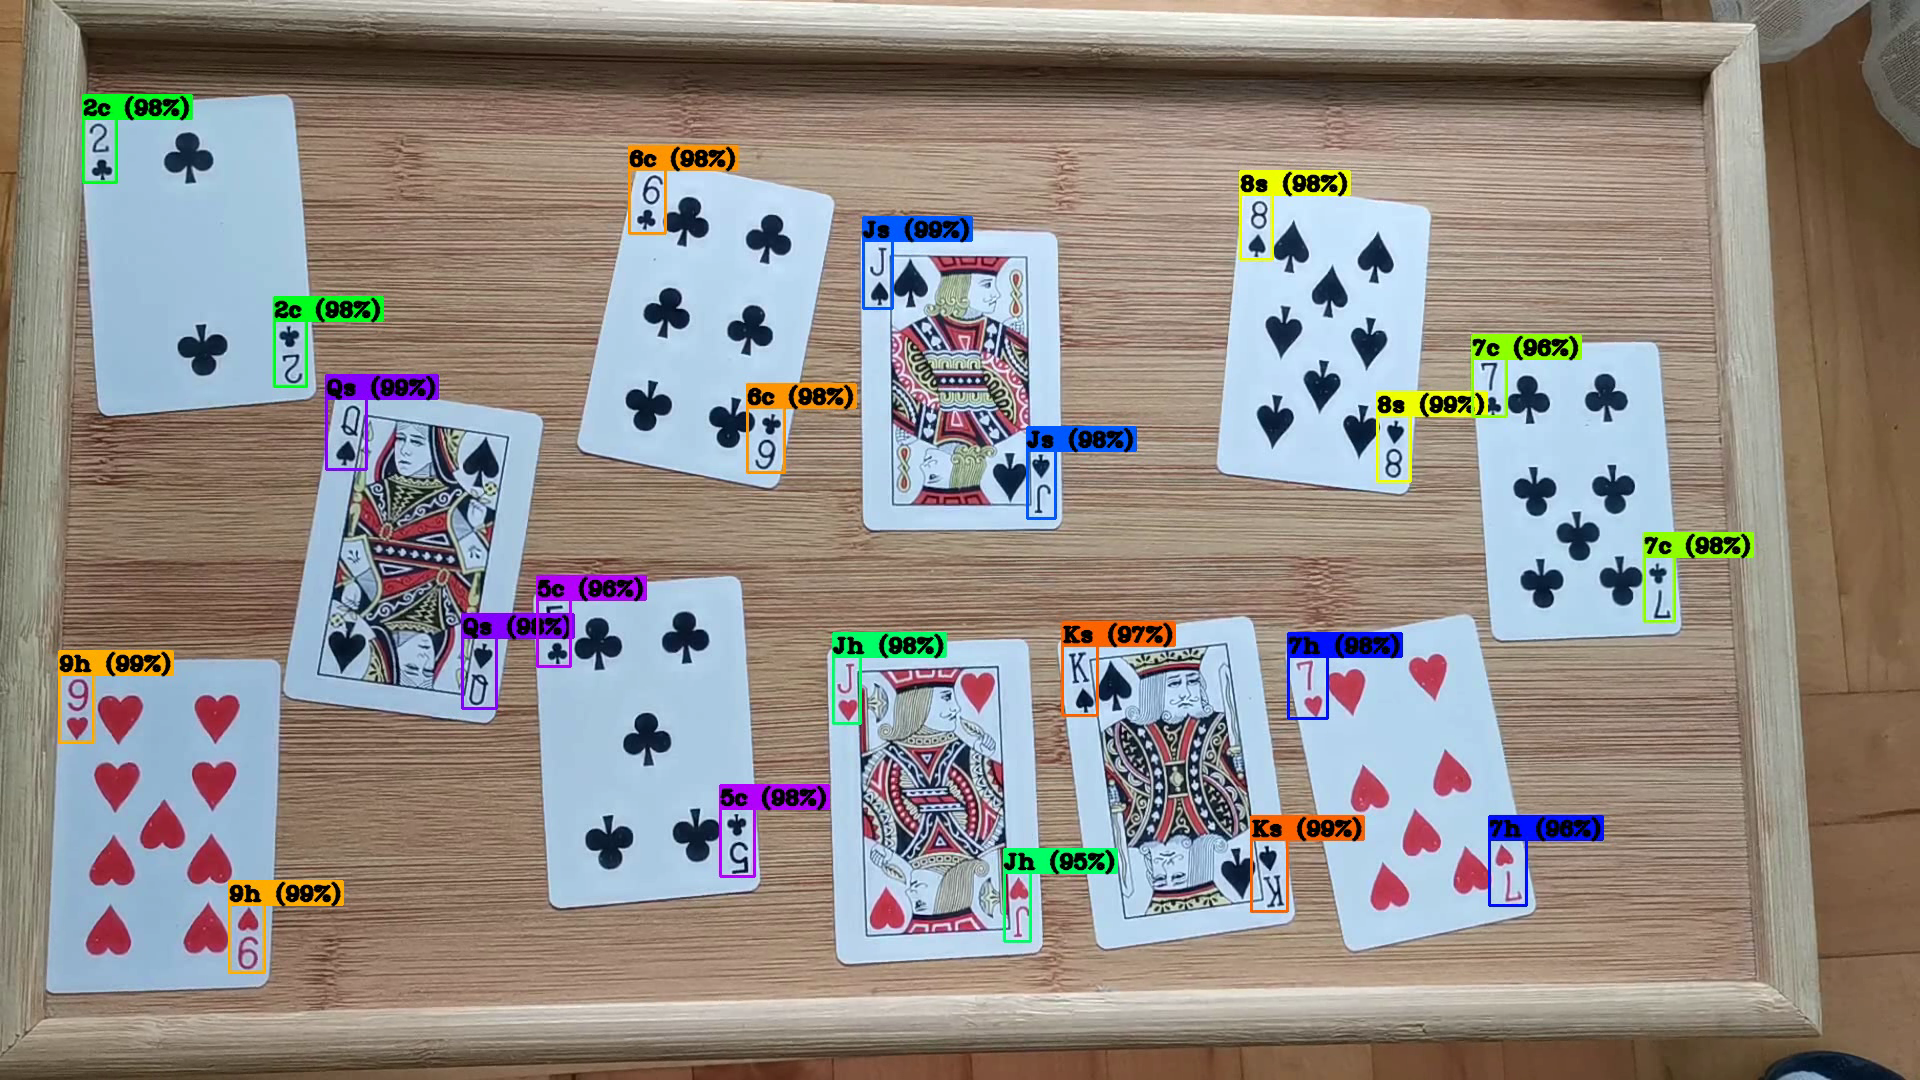
\includegraphics[scale=0.2]{slike/TestVideo.png}
\end{figure}
\end{frame}

\begin{frame}
\frametitle{Промене конфигурација током тренирања}
\begin{itemize}
 \item Тренинг скуп има 50000 слика, а валидациони 10000 (20\%)
 \item \alert{До 3000.\ }итерације је вршено тренирање
 са \alert{већом} вредношћу параметра \mbox{\alert{lerning\ rate=0.001}}
 \begin{itemize}
  \item Mера тачности мреже над тренинг скупом
  (Mean Average Precission - mAP) је била око 97.5\%
  \item При тестирању над видеом \alert{детекције нису биле тачне}
 \end{itemize}
 
 \item После тренирања од \alert{још 400 итерација}, за \alert{финије подешавање},
  са \alert{мањом} вредношћу параметра
  \mbox{\alert{lerning\ rate=0.0001}}
 \begin{itemize}
  \item mAP је износио 100\% над тренинг скупом
  \item На 3400.\ итерацији \alert{резултати} при
  тестирању су били \alert{врло добри}
 \end{itemize}
 
 \item \alert{width} и \alert{height} су постављени на \alert{608}
 (ближе резолуцији камере)
 \begin{itemize}
  \item Тренирање је завршено после извршених \alert{5400} итерацијa
 \end{itemize}
\end{itemize}
\end{frame}

%%%%%%%%%%%%%%%%%%%%%%%%%%%%%%%%%%%%%%%%%%%%%%%%%%%%%%
\section{Закључак}
\begin{frame}
\frametitle{Закључак}
\begin{itemize}
 \item Програм потребно прилагодити физичким објектима
 \item Tренирање траје неколико сати, па резултат
  промене неких конфигурационих параметара није одмах видљив
 \item YOLO (You Only Look Once) извршава детекцијe у једној итерацији
 \item Главни
  аутор рада o YOLO алгоритму, Joseph Redmon
  се повукао са пројекта из етичких разлога
 \item Задивљујућа је чињеница да је сада рачунар
 способан да \textit{види}
 \item Несумњиво је да ће, по речима мог ментора,
\alert{развој Вештачке интелигенције обележити наше каријере}
\end{itemize}
\end{frame}

\begin{frame}[allowframebreaks]{Литература}

\begin{thebibliography}{99}

\bibitem{git_karte}
\textit{playing-card-detection}, приступљено (септембар 2020.) на
\url{https://github.com/geaxgx/playing-card-detection.git}

\bibitem{nn_osnova}
\textit{Machine Learning for Beginners: An Introduction to Neural Networks}, приступљено (септембар 2020.) на
\url{https://towardsdatascience.com/machine-learning-for-beginners-an-introduction-to-neural-networks-d49f22d238f9}

\bibitem{ng}
Andrew Ng, \textit{Convolutional Neural Networks} [Интернет курс], приступљено (септембар 2020.) на
\url{https://www.coursera.org/learn/convolutional-neural-networks/home/welcome}

\bibitem{darknetSajt}
\textit{Darknet: Open Source Neural Networks in C}, приступљено (септембар 2020.) на
\url{https://pjreddie.com/darknet/}

\bibitem{JupyterColab}
\textit{Running a YOLOv4 Object Detector with Darknet in the Cloud! (GPU ENABLED)}, приступљено (септембар 2020.) на
\url{https://colab.research.google.com/drive/1_GdoqCJWXsChrOiY8sZMr_zbr_fH-0Fg?usp=sharing}

\bibitem{YTkarte}
\textit{Playing card detection with YOLO}, приступљено (септембар 2020.) на
\url{https://youtu.be/pnntrewH0xg}

\bibitem{git_moj}
\textit{Diplomski rad - YOLO detekcija}, приступљено (септембар 2020.) на
\url{https://github.com/aleksavelickovic5762015/Diplomski-rad---YOLO-detekcija.git}

\end{thebibliography}

\end{frame}

\end{document}